\documentclass[11pt]{book}

\usepackage[version=digital]{egat}
\makeindex[title=\nombreIdx,intoc]
\logoUniversidad{UNAM_logo}
\logoInstituto{PCF_logo}
\myTitle{Caracterización de pulsos láser debido a una nube de átomos fríos en condiciones de Transparencia Electromagnéticamente Inducida}
\miTitulo{Caracterización de pulsos láser debido a una nube de átomos fríos en condiciones de Transparencia Electromagnéticamente Inducida}
\miNombre{Edgar Giovanni Alonso Torres}
\miUniversidad{Universidad Nacional Aut\'{o}noma de M\'{e}xico}
\miPosgrado{Posgrado en Ciencias Físicas}
\miCampo{Física Cuántica, Atómica y Molecular}
\miAsunto{Protocolo de investigación}
\miGrado{Doctor en Ciencias (Física)}
\miTutor{Dr. Asaf Paris Mandoki (IF-UNAM)}
\miComiteUno{Dr. José Ignacio Jiménez Mier y Terán}
\miComiteDos{Dr. Alfred Barry U'Ren Cortés}
\miCiudad{Ciudad de México,}
\mes{Octubre}
\anio{2024}
\palabrasClave{óptica, cuántica, átomos, Rydberg, interacción, enfriamiento, láser, MOT, presión, cámara}
\metaInformacion

\begin{document}

\renewcommand{\tablename}{Tabla}

\frontmatter
\portada
%\jurado En el paquete quitar las líneas que empiezan en 641 sí se pone jurado

%\begin{dedicatoria}
Para mi hermano y mis papás
\end{dedicatoria}

\begin{agradecimientos}%[\emph{
%La Física es como el sexo: seguro que\\
%da alguna compensación práctica, pero\\
%no es por eso por lo que la hacemos}\\
%\smallskip
%--- An\'{o}nimo
%]
Agradecimientos

\medskip

...

\medskip

Además, agradezco a:

\begin{itemize}
\item El Posgrado de Ciencias Físicas por el apoyo ...
\item CONAHCyT por la beca de doctorado del Programa de Becas Nacionales.
\item Coordinación de Investigación Científica UNAM mediante LANMAC-2020, LANMAC-2021 y LANMAC-2022.
\item DGAPA-UNAM por el apoyo a través del proyecto PAPIIT IA104220.
\item CONACyT con el apoyo mediante los proyectos de Investigación Científica Básica A1-S-29630 y de Laboratorio Nacional 299057, 314860 y 315838.
\end{itemize}

\end{agradecimientos}

\begin{resumen}
....
\end{resumen}

\begin{abstract}
...
\end{abstract}


\tableofcontents
%\listoftables
%\listoffigures

%\begin{Nomenclatura}

{\renewcommand{\arrayrulewidth}{0pt}

\begin{tabular}{@{}C{25mm}L{\textwidth-25mm-2\tabcolsep}@{}}
Símbolo & \multicolumn{1}{c}{Descripción}\\
\cmidrule(lr){1-1}\cmidrule(lr){2-2}
$\A$ & Área de sección transversal\\
$\ell$ & Camino libre medio\\
$\vektor{E}$ & Campo eléctrico\\
$\vektor{B}$ & Campo magnético\\
$A$ & Coeficiente A de Einstein\\
$B_\sm{12},B_\sm{21}$ & Coeficientes B de Einstein\\
$\beta$ & Coeficiente de amortiguamiento viscoso\\
$C$ & Conductancia\\
$k_\sm{\mathrm{B}}$ & Constante de Boltzmann\\
$\kappa$ & Constante de resorte\\
$\varrho$ & Densidad\\
$j_\sm{m}$ & Densidad de caudal de masa\\
$\varphi_\sm{N}$ & Densidad de flujo molecular\\
$\rho(\omega)$ & Densidad espectral de energía\\
$\Delta$ & Desentonamiento\\
$\delta_\sm{+},\delta_\sm{-}$ & Desentonamientos por efecto Zeeman\\
$\mathcal{d}$ & Diámetro\\
$\D$ & Dimensión característica\\
$\V_\sm{\mathrm{N}}$ & Electrodo $\mathrm{N}$ con voltaje igual a $\V_\sm{\mathrm{N}}$\\
$\E$ & Energía\\
$G$ & Factor de ganancia\\
$g$ & Factor de Landé\\
$\phi$ & Fase\\
$\Q$ & Flujo de gas\\
$\omega$ & Frecuencia angular\\
$\Omega$ & Frecuencia de Rabi\\
\end{tabular}

\clearpage

\begin{tabular}{@{}C{25mm}L{\textwidth-25mm-2\tabcolsep}@{}}
Símbolo & \multicolumn{1}{c}{Descripción}\\
\cmidrule(lr){1-1}\cmidrule(lr){2-2}
$\vektor{F}$ & Fuerza, operador de fuerza\\
$\varpsi$ & Función de flujo\\
$H$ & Función de Heaviside\\
$\iH$ & Hamiltoniano\\
$I$ & Intensidad\\
$l$ & Longitud\\
$\lambda$ & Longitud de onda\\
$\mu_\sm{\mathrm{B}}$ & Magnetón de Bohr\\
$m$ & Masa\\
$\vektor{p}$ & Momento, operador de momento\\
$F$ & Momento angular total del acoplamiento espín-espín\\
$J$ & Momento angular total del acoplamiento espín-órbita\\
$\vektor{d}$ & Momento dipolar, operador de momento dipolar\\
$\mu$ & Momento magnético\\
$\mathrm{Kn}$ & Número de Knudsen\\
$\mathrm{Re}$ & Número de Reynolds\\
$\mathrm{Ma}$ & Número Mach\\
$\sigma^\sm{\dagger}$ & Operador de ascenso atómico\\
$\rho$ & Operador de densidad\\
$\sigma$ & Operador de descenso atómico\\
$s$ & Parámetro de saturación\\
$s_\sm{0}$ & Parámetro de saturación en resonancia homogéneo\\
$\hat{\varepsilon}$ & Polarización del campo eléctrico\\
$\sigma_\sm{+},\sigma_\sm{-}$ & Polarizaciones circulares\\
$\vektor{r}$ & Posición, operador de posición\\
$U$ & Potencial\\
$\Phi$ & Potencial eléctrico\\
$P$ & Presión\\
$\Prob$ & Probabilidad\\[-0.17819pt]
$m_\sm{F}$ & Proyección de $F$ sobre el eje de cuantización\\
\end{tabular}

\clearpage

\begin{tabular}{@{}C{25mm}L{\textwidth-25mm-2\tabcolsep}@{}}
Símbolo & \multicolumn{1}{c}{Descripción}\\
\cmidrule(lr){1-1}\cmidrule(lr){2-2}
$m_\sm{J}$ & Proyección de $J$ sobre el eje de cuantización\\
$r$ & Radio\\
$R$ & Resistencia\\
$\gamma_\sm{\perp}$ & Tasa de amortiguamiento transversal\\
$\Gamma$ & Tasa de decaimiento\\
$\gamma_\sm{c}$ & Tasa de decaimiento de coherencia (como colisiones)\\
$\mathcal{g}$ & Tasa de desgasificación\\
$q$ & Tasa de flujo\\
$T$ & Temperatura\\
$\hat{U}$ & Transformación unitaria\\
$\vektor{k}$ & Vector número de onda\\
$\vektor{v},v$ & Velocidad, rapidez\\
$a$ & Velocidad acústica local\\
$S$ & Velocidad de bombeo\\
$u$ & Velocidad de flujo\\
$\bar{c}$ & Velocidad térmica media\\
$\eta$ & Viscosidad dinámica\\
$V$ & Volumen, espacial o de un gas\\
\end{tabular}

}

\end{Nomenclatura}

\mainmatter

\chapter{\label{cap:objetivo}Objetivo general}

En el laboratorio de Óptica Cuántica de Rydberg (OCR), donde estoy realizando mi proyecto de doctorado, queremos crear estados de luz \emph{no clásica} utilizando medios no lineales con ayuda de átomos de Rydberg, lo que denominamos \emph{Óptica Cuántica no lineal de Rydberg}. Este tipo de átomos tienen un electrón excitado en un nivel de energía elevado, lo cual hace que su respuesta a campos externos sea mucho más intensa y de lugar a medios no lineales. Las propiedades de un haz o pulso de luz se modifican por las no linealidades de este tipo de medios, incluyendo la generación de estados no clásicos del campo electromagnético. De la interacción luz-materia podemos investigar, entre otras cosas, dos aspectos relacionados entre sí:

\begin{itemize}
\item[(a)] Las características de un medio a través de la luz.
\item[(b)] Cómo influye un medio conocido en la luz que lo atraviesa.
\end{itemize}

En el caso de (a) para poder ver o, en general, detectar un objeto, éste tiene que sobresalir de sus alrededores. Cuando un objeto destaca por su color o es detectado directamente por las frecuencias de la luz que refleja decimos que es un \emph{objeto de amplitud}, en caso contrario el objeto es transparente pues no refleja ni absorbe la radiación que incide sobre el mismo y lo nombramos \emph{objeto fase}. Lo anterior no excluye el hecho de que estos objetos fase sí modifican la luz, dicha interacción modifica la fase de la radiación que atraviesa el medio. Entonces, podemos obtener información de las propiedades y características de un medio fase a través del cambio de fase que induce el medio en la luz.

\p Mi proyecto de doctorado está centrado en caracterizar los cambios de fase que experimentan pulsos de luz láser debido a un medio fase altamente dispersivo, este medio será una nube de átomos fríos que es transparente a dichos pulsos gracias al fenómeno de \emph{Transparencia Electromagnéticamente Inducida}, que altera sus propiedades ópticas incluyendo el índice de refracción $n_\sm{r}$ y que nos permite tener control en el grado de dispersión $dn_\sm{r}/d\omega$. También medir y cuantificar el cambio en el ancho de los pulsos láser (no ultracortos) y su retraso debido a la dispersión. Además, estos experimentos se realizarán con átomos de Rydberg, con la perspectiva de poder utilizarlos en la generación de estados no clásicos de luz.

\p Caracterizar la luz servirá para, a través de esta, estudiar objetos fase. Conocer un objeto o medio fase tiene su importancia en diversas aplicaciones, tanto en su detección como en mediciones no destructivas donde intencionalmente se utiliza luz que no se absorbe por el medio, esto con la finalidad de no modificar sus propiedades, su dinámica interna o de alterar su estructura como puede ser una muestra biológica. Con mi proyecto espero contribuir al conocimiento en el comportamiento de una nube con átomos de Rydberg en un estado de Transparencia Electromagnéticamente Inducida, dicho medio atómico ha cobrado mucha relevancia en investigaciones de Óptica Cuántica no lineal y de Información Cuántica.

\chapter{\label{cap:introduccion}Introducción}

Diversas áreas de la Física pretenden explicar la materia y la radiación a nivel fundamental, ya sea en el régimen de altas o bajas energías. Ambas áreas buscan nuevos estados o interacciones que arrojen pistas para comprender la Naturaleza, en el estudio a bajas energías es posible utilizar la materia para producir estados no clásicos de luz. Dicha radiación exhibe comportamientos que no se pueden explicar con teorías clásicas, cuando este tipo de situaciones depende de la cantidad de fotones involucrados hablamos de fenómenos de \emph{Óptica Cuántica no lineal}.

\p El estudio de la interacción de medios atómicos no lineales con pocos fotones ha sido de gran interés en las últimas décadas, puesto que los estados no clásico de la luz son ``ladrillos'' para la creación de nuevas herramientas en la Óptica Cuántica y tecnologías en información cuántica~\cite{chen,gorniaczyk,tiarks}, donde queda en evidencia que la luz es excelente para transmitir información mientras que los átomos son un buen medio para procesarla. No obstante, alcanzar no linealidades a nivel de unos cuantos fotones es un reto experimental, por un lado es necesario que dichos fotones interactúen con un mismo átomo determinísticamente y luego que esto modifique el comportamiento del medio, es decir, que algunos átomos afecten todo el conjunto.

\p La probabilidad de interacción puede ser aumentada de dos formas: incrementando el número de fotones o agrandando la sección eficaz de interacción entre fotones y átomos. Lo primero es inconveniente cuando se desean hacer experimentos con fotones individuales, e incompatible si la intensidad de la radiación se vuelve suficientemente alta para producir no linealidades que se explican con modelos clásicos. La segunda opción es desafiante de conseguir en medios usuales, una forma de hacer más grande la sección eficaz es con cavidades de alta fineza, donde los fotones pasan varias veces por los átomos antes de abandonar la cavidad o extinguirse en sus extremos, esto produce una interacción coherente con los átomos~\cite{haroche, birnbaum}. Una desventaja es el tiempo que tarda en salir la luz de la cavidad, mientras que un resonador de baja fineza proporciona monitoreo rápido de su dinámica interna. Usando cavidades de baja fineza cuasi-concéntricas también aumentamos la probabilidad de interacción al reducir el área transversal del láser.

\p En el laboratorio de OCR donde desarrollo mi proyecto de doctorado, además de implementar una cavidad para tener fuertes interacciones entre átomos y fotones, incrementaremos la densidad atómica del medio y aprovecharemos las propiedades de los átomos de Rydberg: átomos con un electrón altamente excitado. Gracias a sus propiedades tan exageradas con el número cuántico principal $n$, la existencia de este tipo de átomos en el medio no sólo amplifica la sección eficaz de cada átomo~\cite{changde}, sino que provee una no linealidad propia al medio, el \emph{bloqueo de Rydberg}: la fuerte interacción entre átomos en estado de Rydberg provoca que exista una vecindad alrededor de los átomos en la cual no es posible excitar otro átomo a estado de Rydberg. La región de bloqueo, cuyo tamaño está en las micras, afecta el comportamiento de los miles de átomos dentro de dicha región.

\p Otro fenómeno a considerar para nuestros experimentos es la transparencia hacia una frecuencia de luz que se induce en los átomos debido a la presencia de un segundo haz de luz que produce interferencia cuántica en las amplitudes de las transiciones ópticas, lo que se denomina como Transparencia Electromagnéticamente Inducida (EIT, por sus siglas en inglés). Una nube de átomos en este escenario es un medio no lineal muy dispersivo que puede generar estados no clásicos de luz~\cite{zhu}. La idea de crear luz no clásica con el bloqueo de Rydberg se planteo en 2005~\cite{friedler}, pero no fue hasta la introducción de EIT que se lograron hacer detecciones no destructivas para medir las interacciones coherentes átomo luz~\cite{mohapatra,dudin,peyronel,maxwell}.

\p Estudiar y cuantificar los cambios que experimentan pulsos de luz que atraviesan átomos fríos en condiciones de EIT es mi proyecto de doctorado, lo cual servirá para caracterizar medios no lineales con los cuales produciremos estados no clásicos de la luz.

\chapter{\label{cap:antecedentes}Antecedentes}

Uno de los propósitos principales del laboratorio de Óptica Cuántica de Rydberg es generar estados no clásicos de luz con átomos de Rydberg, para lograr esto necesitamos de un medio no lineal y analizar la luz que sale de tal medio. En nuestro caso, la no linealidad del medio atómico la obtendremos con el fenómeno de \textbf{Transparencia Electromagnéticamente Inducida} (EIT, por sus siglas en inglés), y mediante \textbf{átomos de Rydberg} incrementaremos las no linealidades. En este capítulo presento brevemente la bases teóricas de EIT, un poco sobre átomos de Rydberg y de óptica cuántica no lineal\miNota{a i a i a i a i a i a i a i a i a i a i a i a i a i a i a i a i a i a i a i a i a i }.

\section{\label{sec:interaccionLuzMateria}Interacción luz-materia}

Gracias a las contribuciones de Planck y la evidencia experimental sobre el comportamiento de la materia sabemos que la energía de los electrones ligados a los átomos es discreta, no pueden adquirir un valor arbitrario de energía como sí lo hacen los electrones libres. Y aún así estos valores discretos o cuantizados, llamados \emph{niveles de energía}, son infinitos. Posteriormente, Schrödinger y contemporáneos proporcionaron las herramientas para resolver y explicar muchas de las observaciones físicas de su época. Si supones que $\phi_\sm{n}(\vektor{r})$ son las funciones propias del Hamiltoniano $\iH_\sm{0}$ para un átomo libre de cualquier campo, entonces la función de onda $\Psi(\vektor{r},t)$ de dicho átomo interactuando con un campo de radiación puede expandir como

\begin{equation}
\label{ec:funcionOndaExpansion}
\Psi(\vektor{r},t)=\sum_{k}c_\sm{k}(t)\phi_\sm{k}(\vektor{r})e^{-j\omega_{k}t}.
\end{equation}

De donde podemos obtener la ecuación de Schrödinger para un átomo interactuando con un campo de radiación~\cite{metcalf}

\begin{equation}
\label{ec:ecuacionSchrodinger}
j\hbar\dfrac{dc_\sm{k}(t)}{dt}= \sum_{l}c_\sm{l}(t)\iH'_\sm{kl}e^{j(\omega_{k}-\omega_{l})t},
\end{equation}

siendo $j$ la unida imaginaria,  $\iH=\iH_\sm{0}+\iH'$ el Hamiltoniano total del sistema y $\iH'_{kl}$ los elementos de matriz del Hamiltoniano de interacción entre el campo y el átomo $\iH'$. Sin embargo, resolver analíticamente la anterior ecuación es imposible, a pesar de que estamos tratando con un solo átomo. Por ello es necesario realizar aproximaciones o simulaciones numéricas.

\subsection{\label{sub:atomo2Niveles}Átomo de dos niveles}

\p Una de los métodos más famosos para tratar la interacción de la luz con un átomo se lo debemos a Rabi~\cite{rabi}, el \textbf{átomo de dos niveles}. Este modelo aborda el problema en un espacio de Hilbert de dimensión reducida, en concreto, uno generado por una base de tan solo dos elementos. Dicha aproximación es válida siempre que las transiciones a otros niveles de energía del átomo sean despreciables y no participan en la dinámica de la interacción. Gracias a este modelo semiclásico podemos explicar diversos comportamientos, tales como las oscilaciones de Rabi, estados vestidos, enfriamiento láser, fluorescencia e incluso la consistencia con otras teorías clásicas, como el modelo de Lorentz (un átomo cuyo electrón está ligado como un oscilador armónico amortiguado) o los coeficientes $A$ y $B$ de Einstein en sus ecuaciones de población de los niveles de energía~\cite{steck2}.

\subsection{\label{sub:atomo3Niveles}Átomo de tres niveles}

\p El siguiente paso de complejidad, al menos en lo que este proyecto respecta, es aumentar a tres la dimensión del espacio de Hilbert, esto es, un \textbf{átomo de tres niveles}. En nuestro caso tenemos dos campos interactuando con el átomo, correspondientes a los láseres que acoplan sus niveles. La especie atómica que utilizamos en los experimentos es rubidio~\cite{rb85,rb87}, los tres estados que están considerados son el estado base $\ket{g}:5\prescript{2}{}{\mathrm{S}}_\sm{1/2}$, el primer estado excitado $\ket{e}:5\prescript{2}{}{\mathrm{P}}_\sm{3/2}$ y otro estado excitado $\ket{r}:n\mathrm{S}$ o $n\mathrm{D}$ según las reglas de selección de transición dipolar. Un láser acopla el estado base con el primer estado excitado y que denominamos láser o \emph{haz de prueba}, el segundo láser va desde el primer estado excitado al otro estado excitado y llamamos \emph{haz de control}, de manera que la configuración de niveles relevantes es la \emph{configuración escalera} (fig.~\ref{fig:configuraciones}). 

\begin{figure}[H]
\centering
\begin{minipage}{0.8\textwidth}
\centering
\includegraphics[width=0.875\textwidth]{configuraciones}
\caption{\label{fig:configuraciones}Configuraciones en las que un átomo de tres niveles puede interactuar con el campo de dos haces láser. De izquierda a derecha son las configuraciones escalera, $\Lambda$ y V. Las energías $\hbar\omega_{1}$ y $\hbar\omega_{2}$ son las energías de transición naturales del átomo, mientras que las frecuencias angulares $\omega_{p}$ y $\omega_{c}$ representan a los láseres de prueba y control, respectivamente. Además, $\Delta_{1}$ y $\Delta_{2}$ son las desintonías netas de la frecuencia de un láser respecto a la frecuencia natural de la transición atómica.}
\end{minipage}
\end{figure}

Bajo las anteriores consideraciones, el Hamiltoniano de este sistema, un átomo de tres niveles interactuando con dos campos de radiación, es $\iH=\iH_\sm{\mathrm{a}}+\iH_\sm{\mathrm{int}}$ donde

\begin{equation}
\label{ec:hamiltonianoAtomico}
\iH_\sm{\mathrm{a}}=\dfrac{\hat{\vektor{P}}^{2}}{2m}+\hbar\omega_\sm{1}\hat{\sigma}_\sm{ee}+\hbar\left(\omega_\sm{1}+\omega_\sm{2}\right)\hat{\sigma}_\sm{rr},
\end{equation}

\begin{equation}
\label{ec:hamiltonianoInteraccion}
\begin{split}
\iH_\sm{\mathrm{int}}= & \hspace{1mm}\dfrac{\hbar}{2}\left[\Omega^{*}_\sm{p}(\vektor{r})e^{-j\left(\vektor{k}_{p}\cdot\vektor{r}-\omega_{p}t\right)}\hat{\sigma}_\sm{ge}+\Omega_\sm{p}(\vektor{r})e^{j\left(\vektor{k}_{p}\cdot\vektor{r}-\omega_{p}t\right)}\hat{\sigma}_\sm{ge}^{\dagger}\right]+\\
& \hspace{1mm}\dfrac{\hbar}{2}\left[\Omega^{*}_\sm{c}(\vektor{r})e^{-j\left(\vektor{k}_{c}\cdot\vektor{r}-\omega_{c}t\right)}\hat{\sigma}_\sm{er}+\Omega_\sm{c}(\vektor{r})e^{j\left(\vektor{k}_{c}\cdot\vektor{r}-\omega_{c}t\right)}\hat{\sigma}_\sm{er}^{\dagger}\right],
\end{split}
\end{equation}

siendo $\omega_\sm{1,2}$ las frecuencias angulares de transición naturales del átomo, $\omega_\sm{p,c}$ las frecuencias angulares de los láseres, $\sigma_{ab}\coloneqq\ketbra{a}{b}$ son operadores de descenso y las frecuencias de Rabi dadas por

\begin{equation}
\label{ec:frecuenciasRabi}
\Omega_\sm{x}(\vektor{r})=\dfrac{\abs{d_\sm{x}}}{\hbar}E_\sm{x}(\vektor{r})e^{j\phi_{x}(\vektor{r})},
\end{equation}

donde $d_\sm{x}$ es el elemento de matriz del operador dipolar atómico $\hat{\vektor{d}}$ correspondiente a la transición acoplada por el campo con intensidad $E_\sm{x}$ y fase $\phi_\sm{x}$. Para incluir procesos no unitarios como el decaimiento espontáneo y decoherencias utilizamos el formalismo de la \emph{matriz de densidad} $\rho$, así la ecuación maestra que rige la dinámica del sistema es

\begin{equation}
\label{ec:ecuacionMaestra}
\dfrac{\partial\tilde{\rho}}{\partial t}=-\dfrac{j}{\hbar}\left[\tilde{\iH},\tilde{\rho}\right]+\Gamma_\sm{e}\D[\hat{\sigma}_\sm{ge}]\hat{\rho}+\Gamma_\sm{r}\D[\hat{\sigma}_\sm{er}]\hat{\rho}+\gamma_\sm{g}\D[\hat{\sigma}_\sm{g}]\hat{\rho},
\end{equation}

con $\Gamma_\sm{e}$ la tasa de decaimiento del estado $\ket{e}$ al estado base $\ket{g}$, $\Gamma_\sm{r}$ la tasa de decaimiento del estado $\ket{r}$ al estado $\ket{e}$. El coeficiente $\gamma_\sm{g}$ toma en cuenta todos los procesos de pérdida de coherencia entre los estados, también está el operador $\hat{\sigma}_\sm{g}\coloneqq\ketbra{g}{g}-\ketbra{r}{r}$ y el súper operador Lindbladiano $\D$~\cite{breuer}.

\subsection{\label{sub:eit}Transparencia Electromagnéticamente Inducida}

A partir de la ecuación maestra (ec.~\ref{ec:ecuacionMaestra}) es posible dar con varios resultados de la interacción entre un átomo y dos láseres considerando sólo tres niveles de energía en la dinámica de sus grados de libertad internos. En particular la respuesta óptica de un medio atómico, es decir, cómo reacciona el medio a campos eléctricos externos.

\p Una da las magnitudes o entidades que contiene la información de la susodicha respuesta óptica es la \emph{susceptibilidad eléctrica} $\chi$, que manifiesta cómo se polariza un medio al aplicar un campo eléctrico debido a sus constituyentes atómicos que actúan como dipolos. La relación entre el campo eléctrico aplicado $ \vektor{E}$ y la polarización del medio $\vektor{P}$ está dada por

\begin{equation}
\label{ec:polarizacionCampoE}
\vektor{P}^\sm{(+)}=\epsilon_\sm{0}\chi\vektor{E}^\sm{(+)},
\end{equation}

suponiendo una respuesta lineal del medio al campo aplicado ($\chi$ un escalar) y el superíndice $(+)$ indica la componente de frecuencia positiva de dicha cantidad, $\vektor{A}=\vektor{A}^\sm{(+)}+\vektor{A}^\sm{(-)}$ con $\vektor{A}^\sm{(-)}=(\vektor{A}^\sm{(+)})^{*}$. En la anterior ecuación $\epsilon_\sm{0}$ es la \emph{permitividad eléctrica del vacío}. Puesto que la susceptibilidad eléctrica está relacionada con el índice de refracción \emph{complejo} $n_\sm{\mathrm{ref}}$ a través de $n_\sm{\mathrm{ref}}=\sqrt{1+\chi}$ para un gas atómico, entonces $\chi$ nos permite conocer el perfil de absorción $\Im{(n_\sm{\mathrm{ref}})}$ y el índice de refracción (real) $n_{r}=\Re{(n_\sm{\mathrm{ref}})}$ del medio en presencia de luz. Para escribir la susceptibilidad eléctrica (cantidad macroscópica) en términos de propiedades atómicas que ya hemos visto, como las tasas de decaimiento o frecuencias de Rabi, es útil recordar que la polarización de un ensamble de átomos está relacionada con el operador de \textbf{momento dipolar} $\hat{\vektor{d}}$ de un átomo mediante su valor esperado:

\begin{equation}
\label{ec:polarizacionMomentoDipolar}
\vektor{P}^\sm{(+)}=n\braket{\hat{\vektor{d}}^\sm{(+)}},
\end{equation}

y $n$ la densidad numérica del conjunto. En el átomo de tres niveles y los dos láseres, el operador de momento dipolar toma en cuenta el acoplamiento del estado base $\ket{g}$ al primer estado excitado $\ket{e}$ y del este último al otro estado excitado $\ket{r}$ (configuración escalera). Lo que nos interesa medir experimentalmente es la respuesta del medio al haz de prueba, por tanto en $\braket{\hat{\vektor{d}}}$ solamente consideraremos el elemento $\braket{g|\hat{\vektor{d}}|e}$ de la componente de frecuencia positiva. Así, la susceptibilidad para el haz de prueba interactuando con un átomo de tres niveles en la configuración escalera está dada por

\begin{equation}
\label{ec:susceptibilidad}
\chi=\dfrac{n\braket{g|\varepsilon_\sm{p}\cdot\hat{\vektor{d}}|e}^{2}}{\hbar\epsilon_\sm{0}}\dfrac{\Delta_\sm{2}+j\left(\Gamma_\sm{r}/2+2\gamma_\sm{g}\right)}{\left[\Gamma_\sm{r}/2+2\gamma_\sm{g}-j\Delta_\sm{2}\right]\left[\Gamma_\sm{e}/2+\gamma_\sm{g}/2-j\Delta_\sm{1}\right]+\Omega^{2}_\sm{c}/4},
\end{equation}

donde $\varepsilon_\sm{p}$ es el vector unitario de polarización del haz de prueba. En la anterior ecuación es importante la configuración que se está considerando, en el caso abordado aquí, si $\delta_\sm{p}$ y $\delta_\sm{c}$ son las desintonías de los haces de prueba y control, respectivamente, | $\Delta_\sm{1}=\delta_\sm{p}$ y $\Delta_\sm{2}=\delta_\sm{p}+\delta_\sm{c}$.

\begin{figure}[H]
\centering
\begin{minipage}{0.8\textwidth}
\centering
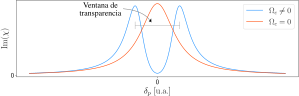
\includegraphics[width=0.875\textwidth]{eit}\\
\includegraphics[width=0.875\textwidth]{dispersion}
\caption{\label{fig:eitDispersion}Las propiedades de un ensamble de átomos se modifican al interactuar con un haz de control resonante. En particular, el medio se vuelve transparente para el haz de prueba en resonancia (gráfica superior) y cambia su índice de refracción (gráfica inferior).}
\end{minipage}
\end{figure}

\p Finalmente, de la ecuación~\ref{ec:susceptibilidad} podemos determinar algunas propiedades macroscópicas. Una de las más interesante emerge cuando el láser de control es resonante con la transición de $\ket{e}$ a $\ket{r}$, es decir, cuando $\delta_\sm{c}=0$ ($\Delta_\sm{1}=\Delta_\sm{2}=\delta_\sm{p}$). En estas condiciones, la interacción del átomo con los campos induce una interferencia entre las vías de excitación, eliminando la absorción en la frecuencia de resonancia de la transición desde $\ket{g}$ a $\ket{e}$. Este fenómeno es la \emph{Transparencia Electromagnéticamente Inducida}~\cite{fleischhauer}, el cual viene acompañado de un medio muy dispersivo~\cite{harris,scully} y que observamos en la figura~\ref{fig:eitDispersion}.

\subsection{\label{sub:luzLenta}Luz lenta}

Que un medio en condiciones de EIT sea altamente dispersivo tiene implicaciones muy interesantes, entre las cuales destaca el cambio en el valor de la velocidad de grupo $v_\sm{g}$ con la cual se propaga un pulso de luz a través de tal medio, velocidad dada por~\cite{harris}	

\begin{equation}
\label{ec:velocidadGrupo}
v_\sm{g}=\dfrac{c}{n_\sm{r}(\omega_\sm{p})+\omega_\sm{p}\dfrac{dn_\sm{r}}{d\omega_\sm{p}}}\approx\dfrac{\hbar c\epsilon_\sm{0}}{2\omega_\sm{p}}\dfrac{\abs{\Omega_\sm{c}}^{2}}{\abs{\braket{g|\varepsilon_\sm{p}\cdot\hat{\vektor{d}}|e}}^{2}n},
\end{equation}

con $\omega_\sm{p}$ la frecuencia angular del haz de prueba. Puesto que la pendiente (gradiente) del índice de refracción alrededor de la resonancia del haz de prueba ($\delta_\sm{p}=0$) se puede hacer muy empinada modificando la intensidad del haz de control, es posible lograr velocidades muy bajas de propagación de hasta 7 órdenes de magnitud por debajo de la velocidad de la luz en el vacío~\cite{hau}. En la ecuación~\ref{ec:velocidadGrupo} vemos que el valor de la velocidad de grupo es proporcional a la intensidad del láser de control $\abs{\Omega_\sm{c}}^{2}$ e inversamente proporcional a la densidad atómica $n$,  significa que es posible alentar la luz entre más denso sea el medio que atraviesa y con menores intensidades, incluso se ha logrado detener efectivamente un pulso de luz al apagar el haz de control~\cite{liu,phillips} y manipular estados de fotones en ensambles atómicos~\cite{lukin1}.

\p Otro aspecto importante del perfil del índice de refracción $n_\sm{r}$ (segunda gráfica en fig.~\ref{fig:eitDispersion}) es que la dispersión de la velocidad de grupo varía según la desintonía del haz de prueba, esto significa que el cambio en el ancho de un pulso que cruce el medio dependerá de la frecuencia del haz de prueba, particularmente en resonancia ($\delta_\sm{p}=0$) el pulso conserva su forma conforme se propaga $\bigl(d^{2}n_\sm{r}/d\omega^{2}=0\bigr)$.

\p Una observación más que podemos hacer es sobre el retraso de la luz, por un lado la densidad atómica modifica la velocidad de propagación en el medio, lo cual retrasa la luz respecto a su velocidad en el vacío, por otro lado el largo o profundidad del medio que atraviesa la luz determina la duración que ésta interactúa con los átomos, incrementando aún más el retraso de dicha luz. Será interesante estudiar la forma y densidad de una nube atómica gracias al retraso en la detección de los pulsos láser.

\subsection{\label{sub:densidadOptica}Densidad Óptica}

Una observación que podemos hacer, como está mostrado en la sección anterior, es que a mayor densidad atómica menor será el valor de la velocidad de grupo, en otras palabras, hay un retraso de la luz que atraviesa el medio respecto a su propagación en el vacío. Además, el largo o profundidad del medio determina la duración que un pulso de luz interactúa con los átomos, incrementando aún más el retraso de la luz. Midiendo el retraso $\Delta t$ de la luz podemos, en principio, determinar la forma y densidad de una nube de átomos puesto que

\begin{equation}
\label{ec:retraso}
\Delta t=L\left(\dfrac{1}{v_\sm{g}}-\dfrac{1}{c}\right),
\end{equation}

donde $L$ es la distancia que recorre la luz dentro del medio. Entonces, utilizar el retraso se convierte en una forma \emph{no destructiva} de caracterizar el medio, puesto que el medio es transparente a los pulsos que enviemos debido al EIT, no hay absorción de fotones y por tanto no hay transferencia de momento que altere la dinámica de los átomos.

\section{\label{sec:atomosRydberg}Átomos de Rydberg}

Como ya mencioné, un átomo posee una infinidad de niveles de energía, resultado del potencial electrostático de Coulomb entre el electrón y los protones del núcleo. Cuando uno de los electrones de un átomo está en un nivel de energía alto, en otras palabras que el número cuántico principal $n$ de dicho electrón es grande, lo denominamos como \textbf{átomo de Rydberg}. Aunque no existe un consenso de que tan grande tiene que ser $n$ para considerar a tal átomo como de Rydberg, es frecuente adoptar $n>20$. Puesto que la interacción entre átomos de Rydberg es muy alta, éstos han han sido útiles en el desarrollo de experimentos de óptica no lineal con fotones individuales~\cite{peyronel,gorniaczyk,chang}.

\p Al estar tan excitado un electrón en un átomo de Rydberg varias de sus características atómicas se modifican, decimos que poseen propiedades exageradas respecto a átomos \emph{ligera} o mínimamente excitados, pues éstas escalan como potencias del número cuántico principal $n$. De entre todos los átomos que existen, los alcalinos son de particular interés al tener un solo electrón de valencia, llevar dicho electrón a un estado muy excitado (estado de Rydberg) lo aleja suficiente del núcleo que la interacción coulombiana se hace efectivamente con un núcleo de una sola carga fundamental ($+1e$) puesto que los electrones restante en las capas cerradas apantallan la carga del núcleo, es decir, que el átomo es esencialmente uno de hidrógeno salvo correcciones. Lo anterior permite estudiar estos átomos con la \emph{teoría del defecto cuántico}~\cite{gallagher,seaton} que aborda estas correcciones debido a la diferencia con el hidrógeno.

\p Otros aspectos ha tener en cuenta es la ``sensibilidad'' de estos átomos a campos eléctricos externos, una consecuencia de lo lejos que está el electrón y por ende débilmente ligado al núcleo. También por ello los tiempos de vida de los estados de Rydberg son hasta cuarto órdenes de magnitud más largos en contraste con estados de poco energía, el orden del tiempo de vida media para los primeros niveles de energía está en los $\si{\nano\second}$, diferente a niveles altamente excitados con tiempos de vida del orden de los $\SI{100}{\micro\second}$. En el artículo de Löw~\cite{low} se resumen algunas propiedades físicas de los estados de Rydberg, en la tabla~\ref{tab:propiedadesRydberg} se presentan unas pocas.

\begin{table}[!ht]
\centering
\begin{minipage}{123.5mm}
\centering
\caption[Escalamiento de algunas propiedades de estados de Rydberg para átomos alcalinos]{\label{tab:propiedadesRydberg}Escalamiento de algunas propiedades de estados de Rydberg para átomos alcalinos. La dependencia en el número cuántico principal efectivo $n^{*}$ es resultado de las características de las funciones de onda para átomos de Rydberg~\cite{gallagher,low}.}
\begin{tabular}{*{3}{l}}
\toprule
\multicolumn{1}{c}{Propiedad} & \multicolumn{1}{c}{Expresión} & \multicolumn{1}{c}{$(n^{*})^{x}$}\\
\cmidrule(lr){1-1}\cmidrule(lr){2-2}\cmidrule(lr){3-3}
Energía de enlace & $\E_\sm{n^{*}}=hcR^{*}/(n^{*})^{2}$ & $(n^{*})^{-2}$\\
Espaciamiento entre niveles & $\E_\sm{n^{*}}-\E_\sm{n^{*}+1}$ & $(n^{*})^{-3}$\\
Radio de órbita & $\braket*{r}=\frac{1}{2}\left[3(n^{*})^{2}-l(l+1)\right]$ & $(n^{*})^{2}$\\
Polarizabilidad & $\alpha_\sm{E}$ & $(n^{*})^{7}$\\
Vida media radiativa & $\tau$ & $(n^{*})^{3}$\\
Momento dipolar de transición & $\abs{\braket{5P||er||n\mathrm{S}}}$ & $(n^{*})^{-3/2}$\\
%Momento dipolar de transición $\abs{\Delta l}=1$ & $\abs{\braket*{nl|er|nl'}}$ & $(n^{*})^{2}$\\
Coeficiente van der Waals & $C_\sm{6}$ & $(n^{*})^{11}$\\
\bottomrule
\end{tabular}
\end{minipage}
\end{table}

\p Para átomos alcalinos la dependencia en el \emph{número} (no entero) \emph{cuántico principal efectivo} $n^{*}=n-\delta_\sm{l}$ contiene la desviación respecto al átomo de hidrógeno a través del \emph{defecto cuántico} $\delta_ \sm{l}$, el cual depende principalmente de la especie atómica y del momento angular orbital $l$. Los estados de momento angular bajo $l$ penetran el núcleo, o dicho de forma más precisa, la función de onda radial de estos estados tienen mayor peso en la región del núcleo, por ende son los estado más perturbados con gran defecto cuántico. Por ejemplo, para el rubidio~\cite{low} se tiene $\delta_\sm{0}=3.13$, $\delta_\sm{1}=2.64$, $\delta_\sm{2}=1.35$, $\delta_\sm{3}=0.016$ y $\delta_\sm{l>3}\approx0$.

\p Los niveles de energía para átomos de Rydberg se pueden obtener de la ecuación radial que obedece la parte radial de la función de onda del electrón de valencia, pues la estructura más compleja del núcleo efectivo (núcleo y electrones internos) no quita la simetría esférica, por lo que la separación usual de variables para la función de onda se mantiene. La parte radial $R(r)=u(r)/r$ obedece

\begin{equation}
\label{ec:funcionOndaRadial}
\left[-\frac{\hbar^{2}}{2\mu}\frac{d^{2}}{dr^{2}}+\frac{l(l+1)\hbar^{2}}{2\mu r^{2}}+V(r)-E\right]u(r)=0,
\end{equation}

en donde $V(r)$ es el potencial debido a la carga nuclear $Z_{0}e$ apantallada por la distribución de carga promediada esféricamente de $N$ electrones internos. Para distancias $r$ suficientemente grandes se da un apantallamiento total, de manera que $V(r)\propto(Ze)^{2}/r$ con $Z=Z_\sm{0}-N$. La energía de enlace que es solución de la anterior ecuación se puede escribir como la expresión de la energía de enlace del hidrógeno

\begin{equation}
\label{ec:energiaEnlace}
\E_\sm{n^{*}}=-\frac{hcR^{*}}{(n^{*})^{2}},
\end{equation}

con $R^{*}=R_\sm{\infty}(1+m_\sm{e}/m_\sm{\text{núcleo}})$, $R_\sm{\infty}=\SI{10973731.568160(21)}{\per\meter}$ la constante de Rydberg. Es posible determinar la función de onda del electrón de valencia tomando en cuenta la estructura fina: la parte angular, al no depender del potencial, queda igual que el caso del hidrógeno, esto es, los \emph{armónicos esféricos de espín}~\cite{cohen}

\begin{equation}
\label{ec:armonicosEsfericosEspin}
Y_\sm{j\pm\frac{1}{2},\frac{1}{2},j,m_{j}}(\theta,\varphi)=\left[2\left(j\pm\dfrac{1}{2}\right)+1\right]^{-\frac{1}{2}}\left(\begin{array}{c}
\mp\sqrt{j\pm\dfrac{1}{2}\mp m_{j}+\dfrac{1}{2}}Y_\sm{j\pm\frac{1}{2},m_{j}-\frac{1}{2}}(\theta,\varphi)\\[5mm]
\sqrt{j\pm\dfrac{1}{2}\pm m_{j}+\dfrac{1}{2}}Y_\sm{j\pm\frac{1}{2},m_{j}+\frac{1}{2}}(\theta,\varphi)
\end{array}\right).
\end{equation}

Mientras que la parte radial, para átomos alcalinos, se puede resolver analíticamente lejos del núcleo, donde el apantallamiento de los electrones internos resulta en un núcleo efectivo de carga $Z=1$, las funciones resultantes se conoce como \emph{funciones de Coulomb}

\begin{equation}
\label{ec:funcionCoulomb}
R_\sm{n^{*},l}(r)=\left(\frac{1}{a_\sm{0}}\right)^{\frac{3}{2}}\frac{1}{\sqrt{(n^{*})^{2}\Gamma(n^{*}+l+1)\Gamma(n^{*}-l)}}W_\sm{n^{*},l+1/2}\left(\frac{2r}{n^{*}a_\sm{0}}\right),
\end{equation}

aquí, $\Gamma(z)$ es la función Gamma y $W_\sm{k,m}(z)$ es la función de Whittaker. La derivación de esta expresión se realiza en la revisión de Seaton~\cite{seaton}.

\subsection{\label{sub:interaccionRydberg}Interacción entre dos átomos de Rydberg}

Además de las propiedades de un átomo de Rydberg individual, en un ensamble de átomos emergen otras que son características de los estados de Rydberg, como lo es el bloqueo de Rydberg (ver~\ref{sub:bloqueoRydberg}). Para comprender estos fenómenos, se estudia la interacción entre dos átomos de Rydberg (que pueden ser diferentes especies químicas), el primer átomo (núcleo $A$ y electrón $1$) separado del segundo (núcleo $B$, electrón $2$) por $\vektor{R}=R\vektor{n}$ (figura~\ref{fig:interaccionRR}) y cuyo hamiltoniano, en la aproximación de Born–Oppenheimer (donde las funciones de onda nucleares y electrónicas se pueden tratar por separado), está dado por

\begin{equation}
\label{ec:hamiltonianoDosAtomos}
\hat{\iH}(\vektor{R})=\hat{\iH}_\sm{0}+\hat{\iH}_\sm{\text{int}}(\vektor{R}),
\end{equation}

\begin{figure}
\centering
\begin{minipage}[c]{0.3\textwidth}
\centering
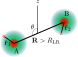
\includegraphics[width=\textwidth]{interaccionRR}
\end{minipage}
\hspace{5mm}
\begin{minipage}[c]{0.4\textwidth}
\centering
\caption{\label{fig:interaccionRR}Sistema de dos átomos de Rydberg cuyo eje interatómico está a un ángulo $\theta$ respecto al eje de cuantización. Las posiciones de los electrones de Rydberg son $\hat{\vektor{r}}_\sm{1}$ y $\hat{\vektor{r}}_\sm{2}$. La distancia interatómica es más grande que el radio de Le Roy $R_\sm{\text{LR}}$, de forma que las funciones de onda electrónicas no se solapen.}
\end{minipage}
\end{figure}

$\hat{\iH}_\sm{0}$ es el hamiltoniano de los estados de Rydberg no perturbados, $\hat{\iH}_\sm{\text{int}}$ engloba la interacción electrostática entre ambos electrones Rydberg, entre ambos núcleos y entre el electrón Rydberg de un átomo con el núcleo del otro átomo.

\p En el marco de esta aproximación, el vector $\vektor{R}$ se trata como un parámetro y no como operador, además su dirección $\vektor{n}$ se toma respecto al eje de cuantización, por lo que es posible escoger un marco donde $\vektor{n}$ se encuentre a un ángulo polar $\theta$ y un ángulo azimutal $\varphi=0$ respecto al eje de cuantización. Tomando en cuenta los términos de estructura fina se tiene que $\hat{\iH}_\sm{0}=\hat{\iH}_\sm{0;1}\otimes\hat{\mathbb{I}}_\sm{2}+\hat{\mathbb{I}}_\sm{1}\otimes\hat{\iH}_\sm{0;2}$ donde

\begin{equation}
\label{ec:hamiltonianoNoPerturbado}
\hat{\iH}_\sm{0;i}=\frac{\hat{\vektor{P}}_\sm{i}^{2}}{2m_\sm{e}}+V(r_\sm{i})-\frac{\hat{\vektor{P}}_\sm{i}^{4}}{8m_\sm{e}^{3}c^{2}}+\left(\frac{Z_\sm{i}e^{2}}{4\pi\epsilon_\sm{0}}\right)\frac{g_\sm{s}}{4m_\sm{e}^{2}c^{2}}\frac{1}{r_\sm{i}^{3}}\hat{\vektor{L}}_\sm{i}\cdot\hat{\vektor{S}}_\sm{i}+\left(\frac{Z_\sm{i}e^{2}}{4\pi\epsilon_\sm{0}}\right)\frac{\pi\hbar^{2}}{2m_\sm{e}^{2}c^{2}}\delta(\hat{\vektor{r}}_\sm{i}),
\end{equation}

con $g_\sm{s}$ el factor de Landé. Los valores valores propios de energía entonces son, hasta primer orden

\begin{equation}
\label{ec:energiaNoPerturnado}
\E_\sm{n,j;i}^{[1]}=-\frac{hcR_\sm{i}^{*}}{n^{2}}\left[1+\frac{(Z_\sm{i}\alpha)^{2}}{n(j+1/2)}-\frac{3(Z_\sm{i}\alpha)^{2}}{4n^{2}}\right],
\end{equation}

y $\alpha$ la constante de estructura fina. Como están involucrados dos átomos, una opción sensata para describir el sistema es utilizar una base construida como el producto tensorial de las bases atómicas individuales $\ket{n_\sm{1}l_\sm{1}j_\sm{1}m_\sm{1};n_\sm{2}l_\sm{2}j_\sm{2}m_\sm{2}}$, donde se hace la omisión usual de los números cuánticos de espín $s_\sm{1}=s_\sm{2}=1/2$ en la notación. De esta forma, cuando $R\to\infty$ la energía de un estado del sistema es simplemente la suma de las energías de átomos individuales, dadas por la ecuación~\ref{ec:energiaNoPerturnado}. Sin embargo, para distancias $R$ lo bastante cercanas, la interacción entre los átomos cambia esto.

\p Si el sistema de referencia se coloca en el núcleo A del primer átomo (figura~\ref{fig:interaccionRR}), y además la distancia interatómica $R$ es suficientemente grande para asegurar que las funciones de onda electrónicas no se solapen, entonces el hamiltoniano de interacción es

\begin{equation}
\label{ec:hamiltonianoInteraccionRydberg}
\hat{\iH}_\sm{\text{int}}(\vektor{R})=\frac{e^{2}}{4\pi\epsilon_\sm{0}}\left(\frac{Z_\sm{1}Z_\sm{2}}{\norm{\vektor{R}}}-\frac{Z_\sm{2}}{\norm{\vektor{R}-\hat{\vektor{r}}_\sm{1}}}-\frac{Z_\sm{1}}{\norm{\vektor{R}+\hat{\vektor{r}}_\sm{2}}}+\frac{1}{\norm{\vektor{R}+\hat{\vektor{r}}_\sm{2}-\hat{\vektor{r}}_\sm{1}}}\right),
\end{equation}

para $R>R_\sm{\text{LR}}$ y donde $R_\sm{\text{LR}}=2\left(\sqrt{\braket{\hat{r}^{2}}_\sm{1}}+\sqrt{\braket{\hat{r}^{2}}_\sm{2}}\right)$ es el \emph{radio de Le Roy}. Al utilizar la base esférica $\vektor{e}_\sm{\pm}=\mp\left(\vektor{e}_\sm{x}\mp i\vektor{e}_\sm{y}\right)/\sqrt{2}$ y $\vektor{e}_\sm{0}=\vektor{e}_\sm{z}$, el hamiltoniano de interacción~\ref{ec:hamiltonianoInteraccion} se puede expresar en su expansión multipolar

\begin{equation}
\label{ec:expansionMultipolar}
\hat{\iH}_\sm{\text{int}}(\vektor{R})=\frac{1}{4\pi\epsilon_\sm{0}}\left[\frac{(1-Z_\sm{1})(1-Z_\sm{2})e^{2}}{R}+\sum_{\kappa=1}^{\infty}\frac{V_\sm{\kappa}}{R^{\kappa+1}}+\sqrt{4\pi}\sum_{\kappa_{1},\kappa_{2}=1}^{\infty}\frac{V_\sm{\kappa_{1},\kappa_{2}}}{R^{\kappa_{1}+\kappa_{2}+1}}\right],
\end{equation}

en donde

\begin{equation}
\label{ec:vectorPotencial}
V_\sm{\kappa}=\sum_{q=-\kappa}^{\kappa}Y_\sm{\kappa,q}^{*}(\vektor{n})\sum_{j=1}^{2}(-1)^{j\kappa}(1-Z_\sm{j})\hat{p}_\sm{\kappa,q}^{(3-j)},
\end{equation}

\begin{equation}
\label{ec:matrizPotencial}
V_\sm{\kappa_{1},\kappa_{2}}=(-1)^{\kappa_{2}}\sum_{q_{1}=-\kappa_{1}}^{\kappa_{1}}\sum_{q_{2}=-\kappa_{2}}^{\kappa_{2}}\frac{Y_\sm{\kappa_{1}+\kappa_{2},q_{1}+q_{2}}^{*}(\vektor{n})}{\sqrt{2(\kappa
_{1}+\kappa_{2})+1}}\sqrt{\binom{\kappa_{1}+\kappa_{2}-q_{1}-q_{2}}{\kappa_{1}-q_{1}}\binom{\kappa_{1}+\kappa_{2}+q_{1}+q_{2}}{\kappa_{2}+q_{2}}}\hat{p}_\sm{\kappa_{1},q_{1}}^{(1)}\hat{p}_\sm{\kappa_{2},q_{2}}^{(2)},
\end{equation}

con $\hat{p}_\sm{\kappa,q}^{(i)}$ los \emph{operadores multipolares esféricos}, dados por

\begin{equation}
\label{ec:operadorMultipolarEsferico}
\hat{p}_\sm{\kappa,q}^{(i)}=e\hat{r}_\sm{i}^{\kappa}\sqrt{\frac{4\pi}{2\kappa+1}}Y_\sm{\kappa,q}(\hat{\vektor{n}}_\sm{i}),
\end{equation}

y $\hat{\vektor{n}}_\sm{i}=(\hat{\theta}_\sm{i},\hat{\varphi}_\sm{i})$ es el operador dirección de $\hat{\vektor{r}}_\sm{i}$.

\p Retomando el caso de átomos alcalinos tenemos $Z_\sm{1}=Z_\sm{2}=1$, por lo cual $V_\sm{\kappa}=0$ para todo valor de $\kappa$. De esta forma, los primeros dos términos de la ecuación~\ref{ec:expansionMultipolar} se anulan:

\begin{equation}
\label{ec:expansionMultipolarAlcalinos}
\hat{\iH}_\sm{\text{int}}(\vektor{R})=\frac{\sqrt{4\pi}}{4\pi\epsilon_\sm{0}}\sum_{\kappa_{1},\kappa_{2}=1}^{\infty}\frac{V_\sm{\kappa_{1},\kappa_{2}}}{R^{\kappa_{1}+\kappa_{2}+1}}.
\end{equation}

Observamos que el hamiltoniano de interacción anterior es una expansión en serie en potencias $\varrho=\kappa_{1}+\kappa_{2}+1$ del inverso de la distancia interatómica. Esta expansión empieza por $\varrho=3$, por lo tanto la contribución de menor orden es la interacción dipolo-dipolo, la cual exhibe la carga neutra de los átomos de Rydberg.

\subsection{\label{sub:intensidadInteraccion}Intensidad de interacción}

Si bien varios experimentos han investigado términos de interacción de orden superior, nosotros restringimos la discusión al término de menor orden, la interacción dipolo-dipolo. En este límite, el hamiltoniano de interacción adopta la forma usual

\begin{equation}
\label{ec:interaccionDipoloDipolo}
\hat{\iH}_\sm{\text{int}}(\vektor{R})=\frac{\hat{\vektor{d}}_\sm{1}\cdot\hat{\vektor{d}}_\sm{2}-3(\vektor{n}\cdot\hat{\vektor{d}}_\sm{1})(\vektor{n}\cdot\hat{\vektor{d}}_\sm{2})}{R^{3}}\eqqcolon\hat{\iH}_\sm{\text{dd}}(\vektor{R}),
\end{equation}

donde $\hat{\vektor{d}}_\sm{i}=e\hat{\vektor{r}}_\sm{i}$. Podemos estudiar este hamiltoniano en dos regímenes, distancias interatómicas pequeñas o grandes, que da lugar a una dependencia $1/R^{3}$ o $1/R^{6}$ en la interacción como se detalla a continuación.

\subsubsection{\label{ssub:resonanciaForster}Intensidad dipolo-dipolo y resonancias de Förster}

La representación en la base esférica del hamiltoniano anterior (ec.~\ref{ec:interaccionDipoloDipolo}) se puede encontrar directamente utilizando $\hat{d}_\sm{j,\pm}=\mp\left(\vektor{d}_\sm{j,x}\pm i\vektor{d}_\sm{j,y}\right)/\sqrt{2}$, o utilizando la expansión~\ref{ec:expansionMultipolarAlcalinos} con $\kappa_\sm{1}=\kappa_\sm{2}=1$. De esta forma, si compactamos la notación como $\ket{1;2}=\ket*{n_\sm{1}l_\sm{1}j_\sm{1}m_\sm{1};n_\sm{2}l_\sm{2}j_\sm{2}m_\sm{2}}$, tenemos que

\begin{equation}
\label{ec:fuerzaDipoloDipolo}
\braket{\hat{\iH}_\sm{\text{dd}}(\vektor{R})}=\braket{1;2|\hat{\iH}_\sm{\text{dd}}(\vektor{R})|1';2'}=\frac{C_\sm{3}(\theta)}{R^{3}},
\end{equation}

siendo $C_{3}(\theta)$ una suma de productos de elementos de matriz radiales y elementos de matriz angulares de ambos átomos del Hamiltoniano total (ec.~\ref{ec:hamiltonianoDosAtomos})~\cite{paris} por factores angulares que provienen del armónico esférico {\color{purple}$Y_\sm{2,q_{1}+q_{2}}^{*}(\vektor{n})=Y_\sm{2,q_{1}+q_{2}} (\theta,0)$} de la ecuación~\ref{ec:matrizPotencial}. La ecuación~\ref{ec:fuerzaDipoloDipolo} representa la intensidad de la interacción entre los átomos de Rydberg, la cual es de tipo dipolo-dipolo debido a la potencia cúbica del inverso de la distancia interatómica.

\p El hamiltoniano dipolo-dipolo $\hat{\iH}_\sm{\text{dd}}$ proporciona el acoplamiento entre diferentes \emph{estados producto} $\ket{1;2}$ y $\ket{1';2'}$, la parte atómica $\hat{\iH}_\sm{0}$ del sistema determina la diferencia de energía inicial $h\Delta_\sm{\text{F}}$ entre dichos estados producto como se muestra en la figura~\ref{fig:defectoForster}; a esta diferencia de energía se le llama \emph{defecto de Förster}. Aun cuando la separación de los niveles de energía para cada átomo ($h\Delta_\sm{1}$ y $h\Delta_\sm{2}$) pueda ser diferente, pueden resultar que el valor del defecto de Förster en la base de estados producto sea pequeño. Si se da tal (casi) resonancia, los niveles involucrados constituyen la contribución dominante de la interacción dipolo-dipolo~\cite{paris}. Así pues, la representación matricial del hamiltoniano, de dimensión infinita, se aproxima por una matriz pequeña donde sólo se involucran estados producto casi resonantes.

\begin{figure}
\centering
\begin{minipage}{0.8\textwidth}
\centering
\includegraphics[width=0.7\textwidth]{defectoForster}
\caption[Defecto Föster]{\label{fig:defectoForster}La estructura de niveles de dos átomos de Rydberg, preparados en $\ket{1}$ y $\ket{2}$, modifica la intensidad de interacción entre estos debido al acoplamiento dipolar a otros estados $\ket{1'}$ y $\ket{2'}$. La interacción se maximiza para defectos de Förster pequeños. Imagen reproducida de~\cite{paris}.}
\end{minipage}
\end{figure}

Las conocidas \emph{resonancias de Förster} ocurren cuando la energía de dos estados producto es degenerada ($\Delta_\sm{\text{F}}=0$), la cual resulta en un acoplamiento resonante entre los estados que conduce a una dependencia \scalebox{0.9}[1]{$\sim$}$1/R^{3}$ de la interacción. En la práctica se habla de resonancias de Förster aun cuando los estados pareja no sean exactamente resonantes, como en el rubidio con los estados pareja $\ket*{41\mathrm{D};49\mathrm{S}}$ y $\ket*{42\mathrm{P};49\mathrm{P}}$~\cite{comparat}.

\subsubsection{\label{ssub:vanderWaals}Fuerza de interacción de van der Waals}

En el caso de que el defecto cuántico sea grande comparado con la intensidad de la interacción $\abs{h\Delta_\sm{\text{F}}}\gg\abs{C_\sm{3}(\theta)/R^{3}}$ (distancias interatómicas grandes), el hamiltoniano de acoplamiento dipolo-dipolo $\hat{\iH}_\sm{\text{dd}}(\vektor{R})$ se puede entender como una perturbación. Es necesario abordar la teoría de perturbaciones a segundo orden, pues la corrección a primer orden de los niveles de energía es

\begin{equation}
\label{ec:perturbacionPrimerOrden}
\Delta\E=\braket*{n_\sm{1}l_\sm{1}j_\sm{1}m_\sm{1};n_\sm{2}l_\sm{2}j_\sm{2}m_\sm{2}|\hat{\iH}_\sm{\text{dd}}(\vektor{R})|n_\sm{1}l_\sm{1}j_\sm{1}m_\sm{1};n_\sm{2}l_\sm{2}j_\sm{2}m_\sm{2}},
\end{equation}

como el operador dipolar $\hat{\vektor{d}}$ no acopla estados de la misma paridad, lo anterior es cero. A segundo orden, la corrección en la energía es

\begin{equation}
\label{ec:perturbacionSegundoOrden}
\Delta\E=\sum_{i,k}\frac{\abs{\braket*{n_\sm{i}l_\sm{i}j_\sm{i}m_\sm{i};n_\sm{k}l_\sm{k}j_\sm{k}m_\sm{k}|\hat{\iH}_\sm{\text{dd}}(\vektor{R})|n_\sm{1}l_\sm{1}j_\sm{1}m_\sm{1};n_\sm{2}l_\sm{2}j_\sm{2}m_\sm{2}}}^{2}}{\E_\sm{1,2}-\E_\sm{i,k}}.
\end{equation}

Observando que el hamiltoniano en la ecuación~\ref{ec:interaccionDipoloDipolo} va como $1/R^{3}$, este término puede salir del valor esperado y la suma en la ecuación de arriba queda

\begin{equation}
\label{ec:fuerzavanderWaals}
\Delta\E=\frac{C_\sm{6}(\theta)}{R^{6}},
\end{equation}

ergo a largas distancias se tiene una interacción de \emph{van der Waals}.

\begin{figure}
\centering
\begin{minipage}{0.8\textwidth}
\centering
\includegraphics[width=0.8\textwidth]{intensidadInteraccion}
\caption{\label{fig:intensidadInteraccion}Intensidad de interacción de dos átomos de Rb en estado base, dos átomos de Rb excitados en $\text{100}\mathrm{S}$ y iones. Imagen reproducida de~\cite{saffman}.}
\end{minipage}
\end{figure}

\subsection{\label{sub:bloqueoRydberg}Bloqueo de Rydberg}

Los elementos de matriz para el hamiltoniano de interacción entre dos átomos están dados en~\ref{sub:intensidadInteraccion}, además de que la parte atómica del hamiltoniano completo proporciona el defecto Förster. En la base de estados producto $\{\ket{1;2},\ket{1';2'}\}$, el hamiltoniano del sistema de dos átomos neutros~\ref{ec:hamiltonianoDosAtomos} queda representado por

\begin{equation}
\label{ec:hamiltonianoCompleto}
\hat{\iH}(\vektor{R})=\begin{pmatrix}
0 & \dfrac{C_\sm{3}}{R^{3}}\\[6mm]
\dfrac{C_\sm{3}}{R^{3}} & \hbar\Delta_\sm{\text{F}}
\end{pmatrix},
\end{equation}

donde $\Delta_\sm{\text{F}}=\Delta_\sm{1}+\Delta_\sm{2}$~(figura~\ref{fig:defectoForster}). La representación matricial anterior es para el caso en el que se define como 0 la energía del estado $\ket{1;2}$, cuyos valores propios de energía son

\begin{equation}
\label{ec:energiasPropias}
\E_\sm{\pm}=\frac{\hbar\Delta_\sm{\text{F}}}{2}\pm\sqrt{\left(\frac{\hbar\Delta_\sm{\text{F}}}{2}\right)^{2}+\left(\frac{C_\sm{3}}{R^{3}}\right)^{2}}.
\end{equation}

Si los átomos no interactúan, la diferencia de energía entre los estados $\ket{1';2'}$ y $\ket{1;2}$ será $\Delta\E_\sm{0}=\hbar\Delta_\sm{\text{F}}$. La interacción dipolo-dipolo entre los átomos modifica la energía de estos estados, que ahora depende de la separación entre los átomos (ec.~\ref{ec:energiasPropias}). La diferencia de energía entre los estados es

\begin{equation}
\label{ec:diferenciaEnergia}
\Delta\E=\E_\sm{+}-\E_\sm{-}=2\sqrt{\left(\frac{\hbar\Delta_\sm{\text{F}}}{2}\right)^{2}+\left(\frac{C_\sm{3}}{R^{3}}\right)^{2}},
\end{equation}

si la interacción es intensa (distancias interatómicas cortas), entonces $\abs{h\Delta_\sm{\text{F}}}\ll\abs{C_\sm{3}(\theta)/R^{3}}$ y los niveles de energía se separan, respecto al caso sin interacción, por

\begin{equation}
\label{ec:diferenciaEnergiasCercano}
\Delta\E_\sm{\text{b}}\coloneqq\Delta\E-\Delta\E_\sm{0}=\frac{2\abs{C_\sm{3}}}{R^{3}},
\end{equation}

mientras que para interacciones débiles $\abs{h\Delta_\sm{\text{F}}}\gg\abs{C_\sm{3}(\theta)/R^{3}}$ (distancias interatómicas grandes), se obtiene

\begin{equation}
\label{ec:diferenciaEnergiasLejano}
\Delta\E_\sm{\text{b}}=\frac{2\abs{C_\sm{3}}^{2}}{\hbar\abs{\Delta_{\text{F}}}R^{6}}=\frac{2C_\sm{6}}{R^{6}}.
\end{equation}

Por supuesto, ambas expresiones deben conciliarse para una distancia intermedia, misma que algunas veces la llaman \emph{radio de van der Waals}. Igualando ambas expresiones~\ref{ec:diferenciaEnergiasCercano} y \ref{ec:diferenciaEnergiasLejano} se concluye que

\begin{equation}
\label{ec:radiovanderWaals}
R_\sm{\text{vdW}}=\sqrt[3]{\frac{\abs{C_{3}}}{\hbar\abs{\Delta_{\text{F}}}}}=\sqrt[6]{\frac{C_{6}}{\hbar\abs{\Delta_{\text{F}}}}}.
\end{equation}

En resumen, la energía de interacción entre dos átomos de Rydberg muestra una fuerte dependencia en el número cuántico principal efectivo $n^{*}$ $\bigl($pues $C_\sm{3}\propto (n^{*})^{4}$, $\Delta_\sm{\text{F}}\propto (n^{*})^{-3}$ y $C_\sm{6}\propto (n^{*})^{11}\bigr)$.

\p En la figura~\ref{fig:bloqueoRydberg} se muestra el cambio de energía del nivel asociado al estado $\ket{1';2'}$ respecto al nivel correspondiente al estado $\ket{1;2}$. Este fenómeno se denomina \emph{bloqueo de Rydberg}, pues aún teniendo dos láseres resonantes con las transiciones de los átomos individuales (uno resonante con $\ket{1}\leftrightarrow\ket{1'}$ y el otro con $\ket{2}\leftrightarrow\ket{2'}$), el cambio de energía debido a la interacción dipolar deja fuera de resonancia el estado $\ket{1',2'}$, siempre y cuando el ancho de línea de la excitación sea más pequeño que el potencial de interacción $2\abs{C_\sm{\beta}}/R^{\beta}$.

\begin{figure}
\centering
\begin{minipage}{0.8\textwidth}
\centering
\includegraphics[width=0.4\textwidth]{bloqueoRydberg}
\caption[Bloqueo de Rydberg]{\label{fig:bloqueoRydberg}Principio del bloqueo de Rydberg entre dos átomos separados una distancia $R$. Cuando los átomos están en el estado $\ket{1';2'}$ interactúan fuertemente, lo cual conduce a un desplazamiento de energía $\Delta\E_\sm{\text{b}}$. Cuando este desplazamiento se hace más grande que $\hbar\Omega_\sm{2}$, el láser queda fuera de resonancia con la transición que acopla el estado de excitación simple con el de excitación doble, y sólo un átomo se puede transferir a un estado de Rydberg a la vez.}
\end{minipage}
\end{figure}

\section{\label{sec:opticaCuantinaNoLineal}Óptica Cuántica no lineal}

El estudio en Óptica es el uso de la materia para manipular a la luz, alterar sus características o propiedades, lo más conocido es el cambio en la amplitud y fase de la luz debido al medio. La interacción se puede exponer de varias maneras, de forma semiclásica como lo describimos en~\ref{sub:atomo3Niveles} y cuyo enfoque es microscópico (descripción de la dinámica de un solo átomo inmerso en un campo de radiación clásico); también está la descripción macroscópica donde consideramos al medio como un todo, sus propiedades son el resultado conjunto de las propiedades de sus constituyentes. Como ya vimos en~\ref{sub:eit}, una de estas propiedades es la polarización $P$ del medio, definida como el momento dipolar promedio por unidad de volumen y que es la respuesta del medio a campos eléctricos externos:

\begin{equation}
\label{ec:polarizacion}
P(t)=\epsilon_\sm{0}\sum_{k\geq1}\chi^{(k)}E^{k}(t),
\end{equation}

donde $\chi^{(k)}$ son las susceptibilidades eléctricas, las cuales dependen completamente del medio. Cuando el valor de $\chi^{(k>1)}$ es despreciable comparado con $\chi^{(1)}$ decimos que el medio es lineal, en caso contrario alguna de las susceptibilidades de orden superior del medio es comparable o mayor a $\chi^{(1)}$ y, por ende, su respuesta es proporcional a alguna potencia del campo eléctrico, lo cual nombramos \emph{Óptica no lineal}~\cite{boyd}. Es posible inducir no linealidades en un medio empleando haces de luz de alta potencia, lo cual es inconveniente en nuestro caso puesto que queremos hacer experimentos a muy bajas intensidades, incluso al nivel de unos cuantos fotones.

\p La \emph{Óptica Cuántica no lineal} se encarga de estudiar la luz y como controlarla usando medios cuyo comportamiento no lineal depende del número de fotones. Las altas no linealidades provocan que la luz interactúe consigo misma, un comportamiento que no sucede normalmente, esto nos provee de mecanismos para crear estados no clásicos de luz~\cite{peyronel,kumlin}.

\subsection{\label{sub:opticaCuanticaNoLinealRydberg}Óptica Cuántica no lineal de Rydberg}

Buscamos convertir pulsos de luz coherente de pocos fotones en luz no clásica mediante el uso de estados de Rydberg, lo que se nombra como \emph{Óptica Cuántica no lineal de Rydberg}~\cite{firstenberg1}. El bloqueo de Rydberg junto con EIT forman una pareja interesante de fenómenos para producir altas no linealidades en un medio atómico, por ejemplo, realizar EIT donde el segundo estado excitado es uno de Rydberg: lejos de resonancia del haz de prueba el medio es opaco, conforme la frecuencia de este láser se hace resonante ingresaremos a la ventana de transparencia de EIT, pero también comenzarán a excitarse los estados de Rydberg generando zonas de bloqueo donde se rompe la condición de EIT. Gracias al bloqueo de Rydberg, un solo fotón altera la dinámica de miles de átomos.

\p Fue a inicios de este milenio cuando surge la idea de utilizar los átomos de Rydberg para crear estados no clásicos de luz~\cite{lukin2}, hecho que reavivo el interés por los átomos de Rydberg. En 2007 se incorpora el fenómeno de EIT para observar la dinámica coherente entre la luz y los átomos~\cite{mohapatra}, evitando la detección destructiva del sistema. Luego se impulsó el uso de átomos de Rydberg para controlar la luz a escala de fotones individuales~\cite{dudin,peyronel,maxwell}.

\p Los fotones, al viajar a través de estos medios no lineales, dan lugar a \emph{polaritones}, una cuasipartícula que es la superposición de una excitación material y radiación electromagnética. Al emplear átomos de Rydberg, su fuerte interacción dipolo-dipolo $\bigl(\alpha_\sm{E}\propto(n^{*})^{7}\text{ y }C_\sm{6}\propto(n^{*})^{11}\bigr.$~tabla~\ref{tab:propiedadesRydberg}$\bigl.\bigr)$ se mapea a los fotones, dicho de otra forma, la componente material de los polaritones dota a estas cuasipartículas la capacidad de interactuar del medio. El estudio de esta interacción de fotones es interesante y se ha utilizado, por ejemplo, para hacer a los fotones atractivos~\cite{firstenberg2} o fotones repulsivos~\cite{cantu}; estos estados de luz claramente son no clásicos puesto que la luz no exhibe estos comportamientos en las teorías clásicas.

\section{\label{sec:rubidio}Rubidio}

La especie atómica que utilizamos es el rubidio (Rb), que al ser un metal alcalino ofrece facilidades en la producción de átomos de Rydberg dada la cantidad de teoría y métodos desarrollados para este tipo de sistemas y su interacción con luz láser. No utilizamos hidrógeno (H) puesto que la transición del estado base al primer estado excitado es ultravioleta, esa misma transición es accesible en el litio Li pero del primer estado excitado a uno de Rydberg es nuevamente ultravioleta; existen técnicas, la tecnología y óptica para esas longitudes de onda, sin embargo, llevar a cabo experimentos de esa naturaleza es más complicado y excesivamente costoso.

\p Los átomos de Rb y cesio Cs son los que poseen transiciones a estados de Rydberg muy accesibles (en el visible), elegimos rubidio por motivos prácticos. En la naturaleza existen dos isótopos del rubidio, a saber $\prescript{85}{}{\mathrm{Rb}}$ y $\prescript{87}{}{\mathrm{Rb}}$, gran parte de sus propiedades físicas son bien conocidas y se resumen en las hojas de datos de Steck~\cite{rb85,rb87}. Tomando en cuenta la estructura fina el estado base del Rb es $5\prescript{2}{}{\mathrm{S}}_\sm{1/2}$ y el primer estado excitado está desdoblado en $5\prescript{2}{}{\mathrm{P}}_\sm{1/2}$ y $5\prescript{2}{}{\mathrm{P}}_\sm{3/2}$ gracias al acoplamiento espín-órbita; la transición $5\prescript{2}{}{\mathrm{S}}_\sm{1/2}\to5\prescript{2}{}{\mathrm{P}}_\sm{1/2}$ ($5\prescript{2}{}{\mathrm{S}}_\sm{1/2}\to5\prescript{2}{}{\mathrm{P}}_\sm{3/2}$) se llama \emph{transición/línea D1} (\emph{transición/línea D2}).

\p La excitación del Rb a otros niveles de energía debe de seguir las reglas de selección de estas transiciones:

 \begin{equation}
\label{ec:reglasSeleccion}
\begin{split}
\Delta L= & \pm1\\
\Delta J= & \hspace{1mm}0,\pm1\\
\Delta F= & \hspace{1mm}0,\pm1\\
\Delta M_\sm{F}= & \hspace{1mm}0,\pm1\\
\Delta F\neq0\text{ si }M_\sm{F}\hspace{0.5mm} & =M_\sm{F'}=0.
\end{split}
\end{equation}

Son estas reglas de selección a partir de las cuales se tienen las líneas D1 y D2. Las dos formas más utilizadas para obtener estados de Rydberg con Rb son:

\begin{equation}
\label{ec:rydbergRb1}
5\mathrm{S}\xrightarrow[]{\SI{780}{\nano\meter}}5\mathrm{P}\xrightarrow[]{\SI{480}{\nano\meter}}n\mathrm{S}/n\mathrm{D},
\end{equation}

\begin{equation}
\label{ec:rydbergRb2}
5\mathrm{S}\xrightarrow[]{\SI{420}{\nano\meter}}6\mathrm{P}\xrightarrow[]{\SI{1016}{\nano\meter}}n\mathrm{S}/n\mathrm{D},
\end{equation}

cuyas frecuencias son del visible o infrarrojo, disponibles con láseres comerciales de diodo cuyo costo es mucho menor que láseres ultravioletas.

\section{\label{sec:laboratorioOCR}Labortatorio de Óptica Cuántica de Rydberg}

El proyecto de doctorado lo llevaré a cabo en el laboratorio de Óptica Cuántica de Rydberg a cargo del Dr. Asaf Paris Mandoki. La meta del laboratorio es realizar y estudiar experimentos de óptica cuántica no lineal con el uso de átomos de Rydberg con la visión de ampliar el conocimiento en interacciones fundamentales entre luz y materia.

\begin{figure}[H]
\centering
\begin{minipage}{0.8\textwidth}
\centering
\includegraphics[width=0.725\textwidth]{sistemaLaseres}
\caption{\label{fig:sistemaLaseres}Sistema actual de láseres para enfriar y atrapar átomos, así como producir átomos de Rydberg. En la mesa óptica se encuentran el láser maestro que es la referencia en frecuencia de los láseres de enfriamiento, rebombeo e imagen. También está el láser azul para las transiciones a estados de Rydberg.}
\end{minipage}
\end{figure}

El surgimiento del laboratorio comenzó en el 2018, durante ese año y el siguiente se realizó el montaje y construcción del sistema de láseres, mismo que sirve para la generación de la luz que es necesaria para efectuar los experimentos deseados. Este sistema ha ido creciendo y crecerá con el tiempo por los requerimientos de los experimentos, a día de hoy el sistema de láseres está conformado de un láser maestro de luz infrarroja ($\SI{780}{\nano\meter}$) anclado en frecuencia a una cavidad de ultra baja expansión (ULE por sus siglas en inglés) con el método de Pound–Drever–Hall~\cite{black} (PDH), sirve de referencia para anclar otros tres láseres: enfriamiento y rebombeo, utilizados para enfriar la nube de átomos (una trampa magneto-óptica, MOT por sus siglas en inglés) y el láser de imagen para obtener información del medio atómico.

\p Otro láser del sistema es el de $\SI{960}{\nano\meter}$, anclado de igual forma a la cavidad mediante PDH, se utiliza para realizar las transiciones del primer estado excitado a un estado superior (ver~\ref{sub:atomo3Niveles}). Se planea instalar un láser de $\SI{1064}{\nano\meter}$ para una trampa dipolar con la cual aumentaremos el número de átomos que se atrapan en la MOT y la densidad de dicho ensamble.

\p Luego, a partir del año 2020 fuimos construyendo el sistema de vacío, así como el montaje optomecánico y de bobinas para la implementación de la MOT~\cite{alonso}. Las condiciones alcanzadas con el vacío, después del proceso de horneado, bombeo y optimización, son una presión interna por debajo de lo $\SI{10e-10}{\milli\bar}$ y temperaturas inferiores a los $\SI{100}{\micro\kelvin}$ del conjunto de átomos atrapados. El sistema de láseres y de vacío nos permitió generar átomos de Rydberg que detectamos con la Transparencia Electromagnéticamente Inducida (fig.~\ref{fig:eit}).

\newsavebox{\avancesBox}
\begin{figure}[!ht]
\centering
\begin{minipage}{0.9\textwidth}
\centering
\sbox{\avancesBox}{\includegraphics[width=0.5\linewidth]{sistemaVacio}}
\subcaptionbox{\label{fig:vacioActual}}[0.45\linewidth]{
\vbox to \ht\avancesBox{
\vfill
\includegraphics[width=\linewidth]{eitExp}
\vfill}}
\hfill
\subcaptionbox{\label{fig:eit}}[0.5\linewidth]{\usebox{\avancesBox}}
\caption[Trabajo en laboratorio de OCR]{\label{fig:eitVacioActual}(a) Medición de EIT en el laboratorio de OCR en un ensamble de átomos de $\prescript{87}{}{\mathrm{Rb}}$ aproximadamente a $\SI{100}{\micro\kelvin}$, el estado de Rydberg de dicha medición fue $28\mathrm{S}$. (b) Actualidad: sistema de vacío y optomecánica requerida para la MOT y los demás haces láser.}
\end{minipage}
\end{figure}

\chapter{\label{cap:objetivosEspecificos}Objetivo específicos}

En el capítulo anterior traté un poco la teoría alrededor de la Transparencia Electromagnéticamente Inducida (EIT), sobre los átomos de Rydberg y como son utilizados para producir medios atómicos con una respuesta no lineal dependiente del número de fotones, medios capaces de transformar estados de luz coherente o clásica a luz no clásica. La meta de mi doctorado es realizar experimentos que consisten en mandar pulsos de haces láser a través de un ensamble de átomos fríos de Rb en condiciones de EIT, medir y caracterizar estos pulsos, como el cambio en su fase o en su ancho. A través del estudio de la luz podremos conocer las propiedades de medios no lineales, ahí la importancia en el análisis de estos pulsos láser. También, aprovechando el fenómeno de luz lenta dentro de estos medios no lineales pretendemos conocer su forma y densidad sin modificar la dinámica interna de los átomos.

%\section{\label{sec:objetivoExperimento}Montaje y realización experimental}
%
%El montaje de la optomecánica necesaria lo realizaremos para poder mandar dos pulsos láser a través del medio en estado de EIT, uno de los pulsos será resonante con la ventana de transparencia del medio mientras que el otro estará desintonizado en frecuencia lo suficiente para que no sea absorbido por el medio. Una vez ambos pulsos láser atraviesen el medio se cambiará la frecuencia del pulso desintonizado para que ambos pulsos tengan la misma frecuencia y poder realizar una detección homodina (ver~\ref{sub:deteccionHomodina}) con el fin de conocer el cambio de fase introducido por el medio.
%
%\p Durante esta etapa optimizaremos la construcción de este sistema de cambio de frecuencias y detección para obtener una señal clara de un cambio de fase en la luz de entrada. Ya hemos hecho avances en una técnica para cambiar la frecuencia de uno de los dos pulsos láser y conocemos la fase relativa que se acumula entre ambos pulsos (ver~\ref{sec:cambiadorFase}).

\section{\label{sec:caracterizacionFase}Caracterización de los pulsos láser}

Cuantificaremos las propiedades de los pulsos láser que salen del medio no lineal, lo haremos utilizando el control que tendremos en lo dispersivo del medio, y por tanto en la velocidad de grupo de propagación de pulsos láser, a través de la intensidad del haz de control y la densidad atómica. Debido a la dispersión esperamos conocer el cambio en la fase de los pulsos y en su ancho, esto lo lograremos con la técnica de detección homodina (ver~\ref{sub:deteccionHomodina}). Además, contrastaremos con simulaciones de la propagación de tales pulsos en medios atómicos de esas características.

\section{\label{sec:medicionLuzLenta}Medición de luz lenta}

Utilizaremos fotodiodos de alta resolución ($\SI{150}{\mega\hertz}$) para medir el retraso que sufre un pulso láser debido a la nube de átomos altamente dispersiva. A través de esta luz lenta pretendemos caracterizar la nube atómica, puesto que la velocidad de grupo depende de la densidad medio, ésta se mapea al retraso de la luz. Al igual que con la fase, variando la intensidad del haz de control cambiamos el valor del retraso, utilizando la ecuación~\ref{ec:velocidadGrupo} conoceremos la densidad del medio y con~\ref{ec:retraso} su espesor, esto sin destruir la nube de átomos debido a procesos de absorción y emisión de fotones.

\chapter{\label{cap:metodologiaTecnicas}Metodología y técnicas}

Con la finalidad de realizar los experimentos pertinentes al proyecto de mi doctorado primero hay que preparar una nube de átomos fríos y generar las condiciones requeridas para tener un medio en condiciones de transparencia electromagnéticamente inducida. También es necesario montar los componentes necesarios para la detección de la imagen con la cual obtendremos información del cambio de fase. Posteriormente está el análisis de los datos que se comparará con simulaciones numéricas para obtener conclusiones.

\section{\label{sec:generacionRydberg}Generación de estados de Rydberg}

La producción de un medio con átomos en estado de Rydberg pasa, primero, por aislar a los átomos de interacciones externas y proporcionar un ambiente controlado. Durante el año 2021, en el laboratorio de Óptica Cuántica de Rydberg OCR (ver~\ref{sec:laboratorioOCR}), se hizo el armado y montaje del sistema de vacío cuya presión interna es menor a $\SI{10e-10}{\milli\bar}$~\cite{alonso}, dentro de la cámara de vacío se encuentran dispensadores que emiten gas de Rb al paso de una corriente en ellos. Esta cámara a ultra alto vacío suprime en gran medida las interacciones del gas de Rb con otras partículas a tal punto que se vuelven despreciables.

\subsection{\label{sub:mot}Trampa Magneto-Óptica}

\begin{wrapfigure}{r}{0.45\textwidth}
\vspace{-2\baselineskip}
\centering
\begin{minipage}{0.42\textwidth}
\centering
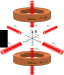
\includegraphics[width=0.65\linewidth]{MOT}  
\caption[Esquema de una MOT]{\label{fig:mot}Trampa Magneto-Óptica. Las bobinas producen un campo magnético cuadrupolar $\vektor{B}$ necesario para atrapar los átomos usando haces láser con la polarización adecuada, circular derecha $\sigma_\sm{+}$ o circular izquierda $\sigma_\sm{-}$.}
\end{minipage}
\end{wrapfigure}

Para enfriar a los átomos implementamos la técnica de \emph{Trampa Magneto-Óptica} (MOT, por sus siglas en inglés) que les valió el premio Nobel de Física a S. Chu, C. Tannougji y W. Phillips en 1997. Esta técnica ennfria una nube de átomos en tres dimensiones espaciales mediante tres pares de haces láser contrapropagantes y ortogonales entre sí. El confinamiento de estos átomos en una región del espacio, dada por la intersección de los seis haces, lo lleva a cabo la luz al interactuar con los átomos, cuya estructura interna está enriquecida por el desdoblamiento de sus niveles magnéticos debido a un campo cuadrupolar generado por un par de bobinas. Bajo estas circustancias podemos describir la interacción luz-materia como una fuerza viscosa que reduce la velocidad de los átomos, a la vez que restauradora que los mantiene atrapados, como si de un resorte se tratara.

\subsection{\label{sub:luzAnclaje}Luz láser y anclaje}

Otro aspecto importante es la estabilidad de los haces láser, tanto en potencia, modo espacial y frecuencia. En el laboratorio de OCR trabajamos con controladores para cada láser que mantiene una temperatura fija para los diodos láser y cuenta con la función de retroalimentación para fijar la frecuencia de los láseres. Entonces, como todo sistema de retroalimentación, es necesario contar con una referencia para su funcionamiento, en este caso una referencia en frecuencia. El sistema de láseres consta actualmente de 5 protagonistas, 4 láseres en el infrarrojo cercano y el quinto de luz azul:

\begin{itemize}
\item \textbf{Enfriamiento}: láser que utilizamos para crear los tres brazos ortogonales de luz de la MOT. Su frecuencia se ancla a la transición hiperfina $F=3\to F'=4$ del $\prescript{85}{}{\mathrm{Rb}}$ $\bigl(F=2\to F'=3\text{ para el }\prescript{87}{}{\mathrm{Rb}}\bigr)$, la cual denominamos \emph{transición de enfriamiento}. Posteriormente se desintoniza al rojo para enfriar los átomos~\cite{foot}.
\item \textbf{Rembombeo}: sintonizado en frecuencia con la transición $F=2\to F'=3$ del $\prescript{85}{}{\mathrm{Rb}}$ $\bigl(F=1\to F'=2\text{ para el }\prescript{87}{}{\mathrm{Rb}}\bigr)$, sirve para reingresar los átomos, cuya población haya pasado al nivel $F=2$ (o $F=1$), a la transición de enfriamiento.
\item \textbf{Imagen}: tiene las mismas características que el láser de enfriamiento salvo que este no se desintoniza, es resonante con la transición del rubidio para generar una imagen de absorción de la nube atómica.
\end{itemize}

\begin{wrapfigure}{l}{0.45\textwidth}
\vspace{-2\baselineskip}
\centering
\begin{minipage}{0.42\textwidth}
\centering
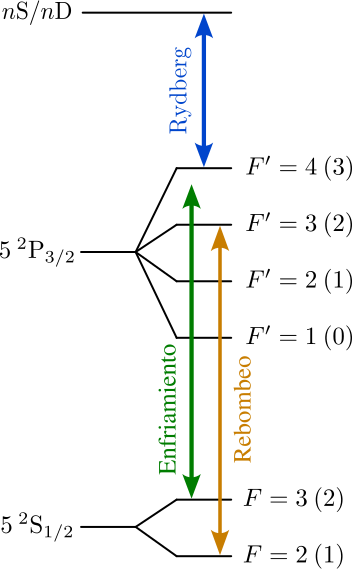
\includegraphics[width=0.65\linewidth]{transiciones}  
\caption[Transiciones del Rb]{\label{fig:transiciones}Transiciones involucradas en la MOT utilizando la línea $\mathrm{D}_\sm{2}$. Sin paréntesis los subniveles de $\prescript{85}{}{\mathrm{Rb}}$ y en paréntesis de $\prescript{87}{}{\mathrm{Rb}}$.}
\end{minipage}
\end{wrapfigure}

Los anteriores láseres se anclan tomando como referencia la frecuencia del que denominamos \textbf{láser maestro}: este láser está anclado en frecuencia a una cavidad mediante el método de Pound-Drever-Hall~\cite{black}, utilizando un modulador electro-óptico somos capaces de anclar el láser maestro a una frecuencia arbitraria y no sólo a las frecuencias del resonador cuya separación está fija por el \emph{rango espectral libre}~\cite{steck1}. El anclaje lo elegimos a la frecuencia del \emph{crossover} $3\otimes4$ del $\prescript{85}{}{\mathrm{Rb}}$ que corresponde a una longitud de onda de aproximadamente $\SI{780.244}{\nano\meter}$.

%en nuestro caso usamos un generador de funciones $f_\sm{\mathrm{GF}}$ y una DDS $f_\sm{\mathrm{DDS}}$ junto con un mezclador electrónico para mandar dos frecuencias a una de las dos entradas de un Modulador Electro-Óptico (EOM, por sus siglas en inglés) $f_\sm{\mathrm{GF}}+f_\sm{\mathrm{DDS}}$ y $\abs{f_\sm{\mathrm{GF}}-f_\sm{\mathrm{DDS}}}$. Si el láser maestro emite luz de la forma $E_\sm{0}=\E_\sm{0}e^{-j2\pi ft}$ que se envía a la otra entrada del EOM, este componente modula la fase del haz de la forma
%
%\begin{equation}
%\label{ec:modulacionFase}
%E=\E_\sm{0}\exp{\left\{-j2\pi\left[f+\beta_\sm{+}\sen{\left(f_\sm{\mathrm{GF}}+f_\sm{\mathrm{DDS}}\right)}+\beta_\sm{-}\sen{\abs{f_\sm{\mathrm{GF}}-f_\sm{\mathrm{DDS}}}}\right]t\right\}},
%\end{equation}
%
%para determinadas constantes $\beta_\sm{\pm}$ llamadas \emph{profundidad de modulación de fase}. Con ayuda de la identidad de Jacobi–Anger expandimos la expresión en la ecuación~\ref{ec:modulacionFase} para concluir que a la salida del EOM tenemos una onda cuyas componentes en frecuencia son: la frecuencia nominal del láser $f$, otras dos a una distancia $f_\sm{\mathrm{DDS}}$ de $f$ que llamamos bandas laterales, y otras cuatro frecuencias que son las bandas laterales de las bandas laterales anteriores y que distan $f_\sm{\mathrm{GF}}$ de estas últimas. Con estas bandas laterales y un resonador óptico podemos fijar la frecuencia del láser maestro a una frecuencia arbitraria y no sólo a las frecuencias del resonador cuya separación está fija por el \emph{rango espectral libre}~\cite{steck1}. El anclaje lo elegimos a la frecuencia del \emph{crossover} $3\otimes4$ del $\prescript{85}{}{\mathrm{Rb}}$ que corresponde a una longitud de onda de aproximadamente $\SI{780.244}{\nano\meter}$.

\p Finalmente tenemos el haz de luz azul que nombramos \textbf{láser de Rydberg}. Este se obtiene como resultado de enviar un haz de luz en el infrarrojo lejano a través de un cristal no lineal que dobla la frecuencia del campo incidente, reduciendo a la mitad la longitud de onda; dicho proceso es conocido como \emph{Generación del Segundo Armónico} (SHG, por sus siglas en inglés). El anclaje de este láser también se hace mediante la técnica de PDH y su controlador nos permite cambiar la frecuencia para elegir el nivel de Rydberg $n\mathrm{S}$ o $n\mathrm{D}$ que queramos excitar.

\section{\label{sec:controlEstadosAtomicos}Control de estados atómicos}

El ancho de línea de un nivel de energía es proporcional a la tasa de transición $\Gamma$, ésta a su vez es proporcional al cuadrado del elemento de matriz dipolar de esa transición según la regla de oro de Fermi. Así pues, de acuerdo con la tabla~\ref{tab:propiedadesRydberg}, el ancho de línea disminuye como $(n^{*})^{-3}$, al igual que el espaciamiento entre niveles de energía adyacentes. Lo anterior significa que los niveles de energía se juntan más y son más delgados entre mayor sea el nivel de Rydberg, por lo tanto, para lograr una situación predecible de los estados de Rydberg que excitamos en los experimentos es indispensable, por un lado, contar con láseres cuyo ancho de línea sea más delgado que el ancho de línea de las transiciones atómicas. Usamos una cavidad de \emph{ultrabaja expansión} (ULE, por sus siglas en inglés) y alta fineza para anclar el láser de Rydberg, de esta forma el ancho de línea de la luz azul para excitar a estados de Rydberg es sumamente delgado ya que se ancla al máximo del pico de transmisión de la cavidad, cuyo ancho completo a media altura (FWHM, por sus siglas en inglés) es del orden de cientos de $\si{\kilo\hertz}$. Según nuestras mediciones~\cite{eduardo}, la fineza y el FWHM de nuestra cavidad ULE para $\SI{960}{\nano\meter}$ es $\mathcal{F}=\SI{13617\pm7}{}$ y $\nu_\sm{\mathrm{FWHM}}=\SI{109.91\pm0.06}{\kilo\hertz}$.

% Anclar el láser al máximo del pico lo hace más delgado que el ancho del pico de transmisión. No podemos medir el ancho de línea del haz de Rydberg, para ello creo recordar que necesitamos una fibra de varios kilómetros de longitud.

\p Por otro lado, necesitamos controlar de mejor manera la población en los estados atómicos, en concreto en los subniveles magnéticos $m_\sm{F}$, pues hay muchos niveles involucrados y esto resulta en una dinámica muy compleja, sumado a que después del enfriamiento y confinamiento con la MOT los átomos no se encuentran, en conjunto, en un estado bien definido. El láser de rebombeo en un ejemplo del control de la población, en este caso, para enfriar eficazmente a los átomos. Sin embargo, la población se distribuye en las diferentes proyecciones $m_\sm{F}$ de la estructura hiperfina de los átomos, en otras palabras, hay varias vías de excitación posible con dos fotones para ir desde el estado base a un estado de Rydberg puesto que tenemos una mezcla estadística de las proyecciones mágnéticas $m_\sm{F}$, en la figura~\ref{fig:transiciones87Rb} ilustramos todos los caminos para una excitación de Rydberg del $\prescript{87}{}{\mathrm{Rb}}$. Es necesario implementar un bombeo óptico para definir muy bien el subnivel magnético de los átomos en nuestros experimentos.

\begin{figure}[H]
\centering
\begin{minipage}{0.8\textwidth}
\centering
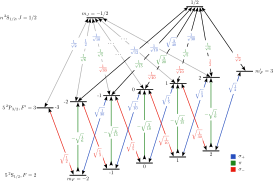
\includegraphics[width=0.8\textwidth]{transiciones87Rb}
\caption{\label{fig:transiciones87Rb}Modelo de átomo de tres niveles en escalera del $\prescript{87}{}{\mathrm{Rb}}$. Se muestran los subniveles magnéticos de la estructura hiperfina para el estado base y el primer estado excitado, para el estado de Rydberg basta considerar la estructura fina.}
\end{minipage}
\end{figure}

\subsection{\label{sub:bombeoOptico}Bombeo Óptico}
 
Utilizaremos \emph{bombeo óptico} para mantener a todos los átomos en un estado de momento magnético bien definido. En presencia de un campo magnético se desdoblan los niveles hiperfinos de los átomos de Rb, es decir, se rompe la degeneración dando lugar a los subniveles magnéticos o niveles Zeeman. Al mandar luz con una frecuencia y polarización definida se van \emph{bombeando} estos subniveles, por ejemplo, con un haz láser para la transición del estado base al primer estado excitado con polarización $\sigma_\sm{+}$, el electrón es bombeado al nivel $m_\sm{F}=2$. La razón está en que la emisión espontánea y estimulada obedece $\Delta m_\sm{F}=0,\pm1$, en el proceso de bombeo el electrón estará en el nivel $m_\sm{F}=2$, cuya transición con el haz polarizado es hacia $m_\sm{F'}=3$ del primer estado excitado, y de este estado sólo puede pasar nuevamente a $m_\sm{F}=2$.

\p Dicho lo anterior, es importante el valor y orientación del campo magnético externo que desplaza los niveles Zeeman, por ello es necesario la construcción de unas bobinas que nos den un valor de campo constante (configuración de Helmholtz) y que al mismo tiempo compensen el campo magnético terrestre.

\section{\label{sec:densidadOptica}Densidad Óptica}

La \emph{Densidad Óptica} $\OD$ de un medio mide su capacidad de reducir la potencia de la luz que lo atraviesa, está relacionada con la transmitancia del medio $T$ por $\OD=-\ln(T)$. Varias medidas experimentales depende del valor de la $\OD$ del medio, en nuestro caso es relevante poder manipular su valor, puesto que la velocidad de grupo y el retraso que experimenta un pulso láser es inversa y directamente proporcional a la densidad óptica del medio, respectivamente.

\p El bombeo óptico que presentamos anteriormente nos ayuda a aumentar la $\OD$ de la nube de átomos, puesto que su probabilidad de excitación es mayor comparado a una nube atómica con una mezcla estadística de los niveles Zeeman.

\subsection{\label{sub:trampaDipolar}Trampa Dipolar}

Sumado al bombeo óptico, una \emph{Trampa Dipolar} servirá para tener control en la $\OD$ de la nube. El principio de funcionamiento de estas trampas está en la interacción dispersiva de la luz con el momento dipolar que ésta induce en los átomos~\cite{grimm}. La fuerza derivada de dicha interacción es conservativa, en contraste con la MOT cuya fuerza es disipativa ya que se usa para enfriar. Entonces, se utiliza el máximo del potencial para atrapar a los átomos, en este caso, el máximo de intensidad del láser $I(\vektor{r})$:

\begin{equation}
\label{ec:fuerzaDipolar}
F_\sm{\mathrm{dip}}(\vektor{r})=\dfrac{1}{2\epsilon_\sm{0}c}\Re{\left(\alpha_\sm{E}\right)}\nabla I(\vektor{r}).
\end{equation}

Con este tipo de fuerza, dependiente del perfil de intensidad del láser, podemos configurar trampas que atrapen a los átomos según el perfil, incluyendo arreglos casi unidimensionales o alargados en una dirección, lo cual aumentará no sólo la densidad atómica sino también la densidad óptica del medio. A su vez, como vimos en~\ref{sub:luzLenta}, el ensanchamiento de la nube en la dirección en la que se propagarán los pulsos de luz incrementará su retraso a la detección.

\section{\label{sec:medicionesFase}Mediciones de fase}

Una forma de cuantificar la interacción entre la luz y la materia es midiendo los cambios que sufre la luz al atravesar el medio atómico, estos cambios se manifiestan en modificaciones de las amplitudes y las fases de las ondas que componen el haz de luz. Monitorear la amplitud se hace de forma directa con la detección de la luz que pasa por los átomos, la corriente registrada en el detector es proporcional a la intensidad de la luz, que a su vez es proporcional al cuadrado de la amplitud; normalizando lo anterior con una medición similar pero sin átomos, es decir, con la amplitud del haz sin modificarse por el medio atómico, obtenemos la \emph{transmitancia} del ensamble de átomos. La transmitancia depende del medio por el cual pasa la luz y existen algunas derivaciones teóricas para modelarlal, como la \textbf{ley de Beer-Lamber}~\cite{bornWolf}, válida para ensambles cuya absorción sea proporcional a su densidad y a la distancia que recorre la luz dentro de estos.

\p Para fines de mi proyecto, lo más interesante está en el cambio en la fase, puesto que queremos medir como responde un haz láser atravesando el conjunto de átomos en condiciones de EIT. Como vimos en~\ref{sub:eit}, el ensamble de átomos se vuelve transparente, por que que la amplitud del campo de la luz no se altera. Lo que es más, la luz atraviesa el medio que es muy dispersivo (gradiente respecto a la frecuencia del índice de refracción). Dado que los detectores solamente pueden medir intensidades, es necesario utilizar técnicas para mapear el cambio de fase a la amplitud del campo y así extraer la información requerida.

\subsection{\label{sub:deteccionHomodina}Detección homodina}

Una técnica para obtener el cambio de fase de una onda es la nombrada \emph{detección homodina}, que consiste en medir la información de fase de un haz láser al compararlo con otro haz de referencia de la misma frecuencia, de ahí su nombre. Se denomina \textbf{señal} al campo de luz cuya fase queremos conocer $E_\sm{\mathrm{S}}(t)$, mientras que el campo de referencia y cuya fase es conocida o se puede controlar muy bien se llama \textbf{oscilador local} $E_\sm{\mathrm{OL}}(t)$.

\begin{figure}[H]
\centering
\begin{minipage}{0.8\textwidth}
\centering
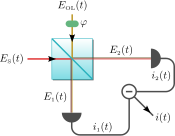
\includegraphics[width=0.4\textwidth]{deteccionHomodina}
\caption{\label{fig:deteccionHomodina}Vista esquemática de la detección homodina. Antes de la detección se controla la fase $\varphi$ del oscilador local y la información de la señal se recupera a partir de la diferencia de las fotocorrientes.}
\end{minipage}
\end{figure}

Ambos haces de entrada se hacen pasar por un \emph{divisor de haz}, los haces de salida $E_\sm{1}(t)$ y $E_\sm{2}(t)$, que son detectados y generan las fotocorrientes $i_\sm{1}(t)$ y $i_\sm{2}(t)$ respectivamente, son el resultado de la superposición de la transmisión de uno de los campos entrantes y la reflexión del otro campo (fig.~\ref{fig:deteccionHomodina}). La relación entre la salida y la entrada se puede expresar con la siguiente ecuación matricial~\cite{saleh}:

\begin{equation}
\label{ec:divisorHaz}
\begin{pmatrix}
E_\sm{1}(t)\\
E_\sm{2}(t)
\end{pmatrix}
=
\begin{pmatrix}
\T & \R'\\
\R & \T' 
\end{pmatrix}
\begin{pmatrix}
E_\sm{\mathrm{OL}}(t)\\
E_\sm{\mathrm{S}}(t)
\end{pmatrix},
\end{equation}

con $\T, \T', \R, \R'$ los coeficientes de transmisión y reflexión del divisor de haz. En general, estos coeficientes son cantidades complejas y son distintos para cada uno de los haces de luz de entrada. Si supones un material que ideal sin pérdidas para el divisor de haz, entonces la intensidad total a la entrada y la intensidad total a la salida es igual, esto es

\begin{equation}
\label{ec:conservacionEnergia}
\abs{E_\sm{\mathrm{OL}}(t)}^{2}+\abs{E_\sm{\mathrm{S}}(t)}^{2}=\abs{E_\sm{1}(t)}^{2}+\abs{E_\sm{2}(t)}^{2}.
\end{equation}

La anterior ecuación de conservación de energía se puede utilizar para probar las siguientes expresiones

\begin{equation}
\label{ec:igualdadModulos}
\abs{\T'}=\abs{\T},\quad\abs{\R'}=\abs{\R},\quad\abs{\T}^{2}+\abs{\R}^{2}=1,
\end{equation}

\begin{equation}
\label{ec:relacionFase}
\T'\R^{*}+\T^{*}\R'=0.
\end{equation}

Las ecuaciones en~\ref{ec:igualdadModulos} relacionan las magnitudes de los elementos de la matriz en~\ref{ec:divisorHaz} para un material sin pérdidas, mientras que~\ref{ec:relacionFase} relaciona sus argumentos. Si ahora también suponemos que el divisor de haz es simétrico, directamente los coeficientes de transmisión y reflexión son iguales y no sólo los módulos como apunta la expresión en~\ref{ec:igualdadModulos}. Con lo anterior obtenemos, a partir de la ecuación~\ref{ec:relacionFase}, que para un divisor de haz simétrico sin pérdidas las fases entre los coeficientes de transmisión $\T=\abs{T}e^{j\phi_{T}}$ y reflexión $\R=\abs{R}e^{j\phi_{R}}$ cumplen que

\begin{equation}
\label{ec:restriccionFase}
\cos{\left(\phi_\sm{T}-\phi_\sm{R}\right)}=0,
\end{equation}

por lo que la fase relativa entre la onda transmitida y la onda reflejada por un divisor de un haz de entrada es de $\pi/2$. Por conveniencia se elige $\phi_\sm{T}=0$, de ahí que la onda reflejada adquiera un cambio de fase $\pi/2$ para garantizar la unitariedad de la matriz de transformación en~\ref{ec:divisorHaz}. Si el divisor de haz es balanceado, es decir, que transmite el $50\%$ de la luz y refleja el otro $50\%$, lo que denominamos divisor de haz $50/50$, entonces $\T=1/\sqrt{2}$, $\R=j/\sqrt{2}$ y utilizando la ecuación~\ref{ec:divisorHaz} tenemos que la diferencia en las fotocorrientes $I(t)\propto\abs{E_\sm{1}(t)}^{2}-\abs{E_\sm{2}(t)}^{2}$ es

\begin{equation}
\label{ec:fotocorriente}
i(t)\propto2\Im{\left[E_\sm{\mathrm{OL}}^{*}(t)E_\sm{\mathrm{S}}(t)\right]}.
\end{equation}

Sean $E_\sm{\mathrm{OL}}(t)=\E_\sm{\mathrm{OL}}e^{j\varphi}e^{j\left(\omega t+\phi_{0}\right)}$ y $E_\sm{\mathrm{S}}(t)=\E_\sm{\mathrm{S}}e^{j\left(\omega t+\phi\right)}$  los campos de entrada de la misma frecuencia, con $\varphi$ la fase que introducimos al oscilador local y que controlamos, entonces la corriente $i(t)$ es
	
\begin{equation}
\label{ec:fotocorrienteFase}
i(t)\propto2\E_\sm{\mathrm{OL}}\E_\sm{\mathrm{S}}\sen{\left(\phi-\phi_\sm{0}-\varphi\right)},
\end{equation}

por ende, al conocer la fase del oscilador local y variar la fase $\varphi$ es posible conocer la fase de la señal con un ajuste a la función de fotocorriente $i(t)$ detectada.

\subsection{\label{sub:contrasteFase}Contraste de fase}

Otro método para conocer el cambio de fase que sufre una onda al cruzar un medio transparente es la \emph{imagen por contraste de fase}, que es uno de varios métodos dispersivos para medir fases. En esta sección abordaremos este método y veremos que puede ser visto como un  caso particular de detección homodina. Supongamos un medio transparente en $z=0$, una onda plana que se propaga en la dirección $z$ y cuya expresión justo antes del medio $z\to0^{-}$ es $E_\sm{i}(z\to0^{-},t)=\E_\sm{0}\cos{\left(\omega t\right)}$, el medio induce en la onda una fase dependiente de la posición $\phi(x,y)$, resultando en una onda de fase modulada:

\begin{equation}
\label{ec:ondaFaseModulada}
\begin{split}
\left.E_\sm{\mathrm{FM}}\left(\vektor{r},t\right)\right|_\sm{z=0}= & \hspace{1.5mm}\E_ \sm{0}\cos{\left[\omega t+\phi(x,y)\right]}\\
& \hspace{1.5mm}\E_\sm{0}\cos{\left(\omega t\right)}\cos{\left[\phi(x,y)\right]}+\E_\sm{0}\sen{\left(\omega tx\right)}\sen{\left[\phi(x,y)\right]}.
\end{split}
\end{equation}

Observamos que la expresión en~\ref{ec:ondaFaseModulada} es una onda de amplitud constante, suponiendo que las aberraciones del sistema de imagen (lentes y otros elementos ópticos) es despreciable, entonces el campo en el plano conjugado de imagen es esencialmente el mismo que en~\ref{ec:ondaFaseModulada}. Además, para valores pequeños de $\phi(x,y)$ y utilizando la segunda forma en la ecuación~\ref{ec:ondaFaseModulada} tenemos

\begin{equation}
\label{ec:ondaFasePequena}
E_\sm{\mathrm{FM}}\left(x,y,t\right)=\E_\sm{0}\cos{\left(\omega t\right)}+\E_\sm{0}\phi(x,y)\sen{\left(\omega t\right)},	
\end{equation}

el segundo término en la ecuación de arriba depende del medio pero el primer término no lo hace, es decir, es la parte no dispersada por el medio. Si logramos cambiar la fase relativa entre estos términos exactamente por $\pi/2$, cambiando el coseno a seno (o viceversa):

\begin{equation}
\label{ec:ondaFaseAmplitud}
E_\sm{\mathrm{FM}}\left(x,y,t\right)=\E_\sm{0}\left[1+\phi(x,y)\right]\sen{\left(\omega t\right)},	
\end{equation}

la cual es una onda de amplitud modulada cuya intensidad es proporcional a $1+2\phi(x,y)$, ergo podemos conocer el cambio de fase debido a un medio transparente midiendo la amplitud de la onda que resulta de cambiar por $\pi/2$ la fase, en este caso, de la porción de onda que no se dispersa. Para conseguir lo anterior se utiliza una \emph{lámina de fase}, una placa de un material transparente e índice de refracción $n_\sm{g}$, ésta se coloca en el plano de Fourier~\cite{hecht} del sistema de imagen para cambiar la fase de la luz no dispersada, dependiendo de la composición particular del sistema de imagen será la forma de la lámina de fase. Para una onda plana y una única lente, la porción que no es dispersada se enfoca en el plano de Fourier, una lámina de fase en cuyo centro haya una hendidura de una distancia $d$ tal que el $\left(n_\sm{g}-1\right)d=\lambda_\sm{0}/4$ basta para lograr el cambio de fase deseado. Otra forma es una onda plana que atraviesa un diafragma anular a la entrada del sistema de imagen, en el plano de Fourier la parte no dispersada forma igualmente un anillo, siendo está la forma que ha de tener una lámina de fase en tal sistema~\cite{hecht}.

\p Este método de imagen puede considerarse una detección homodina en cierto sentido, en la cual la luz no dispersada es el oscilador local y la señal el campo de radiación dispersado, donde se introduce una fase $\pi/2$ al oscilador local. Las diferencias que existen entre ambos métodos es que en la imagen por contraste de fase no hay un divisor de haz y se utiliza un solo detector.

\section{\label{sec:luzLentaDeteccionNoDestructiva}Luz lenta y detección no destructiva}

Aprovecharemos que la luz es \emph{lenta} dentro del medio atómico (ver~\ref{sub:luzLenta}) para medir el retraso de pulsos láser y caracterizar dicho medio, puesto que este retraso depende de la profundidad de la nube atómica y la velocidad de propagación en el medio. Utilizaremos un fotodiodo para detectar los pulsos de luz, primero sin átomos atrapados ($v_\sm{g}=c$) y luego con la nube altamente dispersiva en condiciones de EIT. Dado que el espectro de frecuencias de un pulso de luz con perfil temporal cuadrado es muy grande, pues son necesarias demasiadas frecuencias para reconstruirlo, la dispersión del medio afecta de forma distinta el retraso del pulso dependiendo de su componente en frecuencia, como resultado es muy complicado dar un valor preciso al retraso del pulso. Por lo anterior, los pulsos de luz se mandarán con un perfil temporal gaussiano para reducir el número de frecuencias requeridas para reconstuirlos.

\p Para efectuar mediciones verdaderamente no destructivas de la nube de átomos y caracterizarla, mandaremos dos pulsos láser, uno en resonancia dentro de la ventana de transparencia (fig.~\ref{fig:eitDispersion}), que será el pulso de luz lenta, y otro muy fuera de resonancia para que no sea absorbido ni dispersado por los átomos. Para un pulso con una velocidad de grupo de $v_\sm{g}=\SI[per-mode=symbol]{1000}{\meter\per\second}$ y una nube de $L=\SI{500}{\micro\meter}$ de profundidad, el retraso es alrededor de $\Delta t=\SI{500}{\nano\second}$ (ec.~\ref{ec:retraso}), por lo tanto un fotodiodo con un ancho de banda de $\SI{150}{\mega\hertz}$, como los que tenemos en el laboratorio, puede resolver estas diferencias temporales.

\chapter{\label{cap:avances}Avances}

Los avances que se han realizado en relación a mi proyecto son los siguientes.

\section{\label{sec:bobinasBombeoOptico}Bobinas del bombeo óptico}

Como ya mencioné, con el fin de compensar el campo magnético terrestre a la vez de generar el campo para romper la degeneración de los niveles Zeeman, necesitamos bobinas alrededor de los experimentos.

La compensación del campo terrestre se hace con tres pares de bobinas, su diseño estuvo a cargo de un compañero del laboratorio. Un par de bobinas se alinean de manera que compartan el mismo eje axial, la corriente eléctrica que se suministra se manda para que circule en la misma dirección en ambas bobinas, si la separación entre éstas es similar a algún tamaño característico de una bobina (por ejemplo, el radio en bobinas circulares) entonces el campo magnético alrededor del eje axial y entre ambas bobinas es constante, lo que se denomina como \emph{configuración de Helmholtz}. Con el uso de tres pares de bobinas en dicha configuración, y dispuestas de tal forma que sus ejes axiales sean ortogonales entre sí, podemos tener un campo magnético constante en una dirección arbitraria deseada y compensar así el campo de la Tierra. En la figura~\ref{fig:bobinasBombeoOptico} se muestran estas bobinas.

\p Aunque la construcción y montaje de las bobinas ya está realizado, no las hemos calibrado para compensar el campo terrestre, nos falta un circuito electrónico para modificar la corriente en las bobinas rápido entre mediciones experimentales. El técnico académico del laboratorio ya se encarga de su elaboración. Aún así, hemos aprovechado estas bobinas para modificar el campo cuadrupolar necesario para la trampa MOT: debido a los desperfectos experimentales como la alineación de la optomecánica o el lugar donde están colocadas las bobinas de la MOT, el centro del campo cuadrupolar no está necesariamente alineado con el centro de la zona que define el cruce de los tres brazos de luz de la MOT, como consecuencia la temperatura de los átomos en la MOT incrementa debido al desbalance de fuerzas.

\newsavebox{\bobinasBox}
\begin{figure}[!ht]
\centering
\begin{minipage}{0.8\textwidth}
\centering
\sbox{\bobinasBox}{\includegraphics[width=0.4\linewidth]{bobinasBombeoOptico}}
\subcaptionbox{\label{fig:fotoExp}}[0.55\linewidth]{\usebox{\bobinasBox}}
\hfill
\subcaptionbox{\label{fig:bobinasBombeoOpticoDestacado}}[0.4\linewidth]{
\vbox to \ht\bobinasBox{
\vfill
\includegraphics[width=\linewidth]{bobinasBombeoOpticoDestacado}
\vfill}}
\caption[Bobinas del Bombeo Óptico]{\label{fig:bobinasBombeoOptico}(a) Fotografía del sistema de vacío con parte de la optomecánica para formar los haces de la MOT. (b) Imagen donde se resaltan las bobinas del bombeo óptico. Los tres pares de bobinas son ortogonales entre sí.}
\end{minipage}
\end{figure}

Entonces, el campo constante de las bobinas del bombeo óptico nos deja ajustar el cero del campo de atrapamiento para empatarlo con los haces de la MOT, de esta manera el enfriamiento se hace con mayor eficiencia. En adición a las bobinas, usamos otro proceso de enfriamiento independiente de la MOT: una vez ha transcurrido el tiempo característico de carga de la MOT, desintonizamos la luz de los haces de enfriamiento todavía más hacia el rojo y disminuimos su potencia con una rampa de $\SI{1}{\milli\second}$ de duración. La combinación de este proceso con el ajuste del campo nos permite obtener nubes de átomos con temperaturas alrededor de los $\SI{10}{\micro\kelvin}$, un orden de magnitud mejor a situaciones previas.

\section{\label{sec:medicionesEIT}Mediciones de EIT}

Otro avance en el laboratorio fue la generación de la ventana de transparencia en los átomos debido al fenómeno de EIT, la figura~\ref{fig:esquemaEIT} es un esquema del montaje que hay en el laboratorio para esta medición . Lo logramos con un estado de Rydberg $28\mathrm{S}_\sm{1/2}$ del $\prescript{87}{}{\mathrm{Rb}}$. Antes de iniciar mi doctorado ya habíamos logrado producir EIT en nuestra nube de Rb, en lugar de hacer una detección del perfil de intensidad con una cámara CCD (como lo hacíamos aún más antes) utilizamos un contador de fotones (en concreto un SPCM, por sus siglas en inglés) con el objetivo de mejorar la señal a ruido, es decir, en la detección lo que tenemos es un histograma con las cuentas de fotones que llegan al contador. La intensidad del haz de prueba tiene que ser del orden de los $\si{\pico\watt}$ para no quemar el SPCM, nosotros establecemos una media de un millón de fotones por segundo.

\begin{figure}
\centering
\begin{minipage}{0.8\textwidth}
\centering
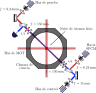
\includegraphics[width=0.8\textwidth]{esquemaEIT}
\caption{\label{fig:esquemaEIT}Esquema del montaje experimental con el que conseguimos excitaciones de Rydberg del Rb y la transparencia EIT. Los haces de prueba y de control son contrapropagantes y con intensidades muy diferentes, del orden de $\si{\pico\watt}$ la intensidad del láser de prueba y de $\si{\milli\watt}$ el haz de control.}
\end{minipage}
\end{figure}

\p El procedimiento que usamos para hacer mediciones del perfil EIT es el siguiente: se enfrían los átomos mediante la MOT para luego apagarla, dejando en caída libre la nube de átomos mientras se expande durante $\SI{100}{\micro\second}$. Inmediatamente después, y por $\SI{100}{\micro\second}$, prendemos la luz de prueba ($\delta_\sm{p}$) y de control (resonante) para realizar EIT, los fotones del láser de prueba que atraviesan el medio atómico son contabilizados por el SPCM. Nuevamente, dejamos caer la nube y a los $\SI{20}{\milli\second}$ volvemos a prender los haces para medir el número de fotones que pasan en ausencia de los átomos. El cociente de estas medidas nos da la transmitancia asociada al medio para la desintonía $\delta_\sm{p}$ del haz de prueba elegido, al repetir las mediciones para diferentes desintonías obtenemos el perfil de absorción de la nube.

\section{\label{sec:cambiadorFase}Cambiador de fase con dispositivos acusto-ópticos}

Dados los objetivos experimentales del laboratorio de OCR necesitamos controlar de forma muy precisa la fase de la luz: no sólo queremos producir estados no clásicos de luz, también queremos caracterizarlos y reconstruirlos a partir de las mediciones que realicemos. Con esto en mente se ideo un dispositivo para controlar la fase de la luz modulando su frecuencia, la razón detrás de esto es la precisión que tenemos en conocer y cambiar frecuencias. Llevamos a cabo el montaje y realización experimental con este susodicho dispositivo, el análisis de los resultados para cambiar la fase y la originalidad de hacerlo con aparatos acusto-ópticos resulto en su publicación en mayo de este año, con el título \emph{High-precision frequency-controlled optical phase shifter with acousto-optic devices}~\cite{esquivel}.

\p Nuestro dispositivo es, en esencia, un interferómetro Mach-Zehnder, la diferencia es que en lugar de modificar activamente la fase de la luz en uno de los brazos, introduciendo un objeto para modificar el camino óptico, cambiamos la frecuencia de uno de los brazos. Durante su propagación la fase relativa entre ambos brazos cambia gracias a que tienen frecuencias diferentes, y justo antes de la detección las frecuencias se vuelven a igualar para que interfieran los haces.

\begin{figure}
\centering
\begin{minipage}{0.8\textwidth}
\centering
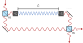
\includegraphics[width=0.8\textwidth]{principioFuncionamiento}
\caption{\label{fig:principioFuncionamiento}Principio de funcionamiento del cambiador de fase. Un haz láser pasa por un divisor de haz 50/50 (BS, por sus siglas en inglés). Uno de los brazos del interferómetro se propaga una distancia $L$ con un cambio de frecuencia sintonizable $f_\sm{S}$. El resultado es un cambio de fase efectivo con respecto al brazo que conserva la frecuencia inicial. Al final se recombinan con otro BS para analizar el cambio de fase mediante el cambio en el patrón de interferencia.}
\end{minipage}
\end{figure}

\p La figura~\ref{fig:principioFuncionamiento} esquematiza el funcionamiento de nuestro dispositivo. Usamos un divisor de haz para crear ambos brazos del interferómetro, la luz de uno de los brazos viaja una distancia $L$ con la frecuencia modificada, luego se regresa a su frecuencia inicial y con otro divisor de haz se recombinan los haces. La distancia $L$ está fija, sin embargo, al cambiar la frecuencia también lo hace el número de longitudes de onda que caben en $L$, esto deriva en una fase extra $\phi=2\pi n_\sm{r}Lf_\sm{S}/c$ con $f_\sm{S}$ la frecuencia que se añadió. El cambio de fase con esta técnica es proporcional al cambio de frecuencia.

\p Con este dispositivo podre realizar el análisis del cambio de fase de la luz que pasa por un medio en condiciones de EIT (ver~\ref{cap:plan}) así como medir cuadraturas del campo electromagnético para la reconstrucción de estados no clásicos de la luz.

\section{\label{sec:retrasoLuz}Medición del retraso de la luz}

Ya hemos realizado experimentos en condiciones de EIT para medir el retraso de la luz, sin embargo, utilizamos pulsos de luz con un perfil temporal cuadrado y no fuimos capaces de resolver si había o no retraso. Hasta ahora se ha desarrollado el programa para que un generador de funciones nos proporcione pulsos con perfil temporal gaussiano.

\chapter{\label{cap:plan}Plan de trabajo}

Lo siguiente en el desarrollo de mi protocolo es el montaje del cambiador de fase alrededor de la cámara de ciencia, la implementación de la trampa dipolar, optimizar las mediciones y realizar el análisis para caracterizar los pulsos de luz que pasan por un medio en EIT, finalmente comparar con simulaciones.

\section{\label{sec:montajeCambiadorFase}Montaje del cambiador de fase}

Utilizando el cambiador de fase podremos mandar, a la vez, dos pulsos de luz que atraviesen el medio atómico. La figura~\ref{fig:montajeCambiadorFase} muestra el plan de montaje de la optomecánica de nuestro dispositivo cambiador de fase con moduladores acusto-ópticos. Primero enviamos un haz a nuestro dispositivo, cuya frecuencia es la misma que la frecuencia del estado base al primer estado excitado del Rb, se crean los dos brazos de luz del interferómetro, uno de ellos con la frecuencia cambiada; luego ambos haces se acoplan a la misma fibra óptica que los manda hacia la nube de átomos en condiciones de EIT, el haz con la frecuencia inicial experimenta la dispersión del medio pues su frecuencia está dentro de la ventana de transparencia (fig.~\ref{fig:eitDispersion}), mientras que al otro haz le cambiamos la frecuencia lo suficiente para que esté suficientemente alejado de dicha ventana y que no sea absorbido por el medio. Una vez pasan el medio, ambos haces se acoplan a otra fibra que los dirige a la segunda parte del dispositivo cambiador para regresar a la frecuencia inicial. Entonces realizamos mediciones de detección homodina.

\begin{figure}[H]
\centering
\begin{minipage}{0.91\textwidth}
\centering
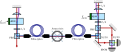
\includegraphics[width=0.95\textwidth]{montajeCambiadorFase}
\caption{\label{fig:montajeCambiadorFase}Plan para implementar nuestro dispositivo cambiador de fase. En este montaje ambos brazos del interferómetro siguen el mismo camino y la nube atómica introduce un cambio de fase en el haz cuya frecuencia está en la ventana de transparencia EIT.}
\end{minipage}
\end{figure}

\section{\label{sec:trampaDipolar}Trampa dipolar}

En la dirección de incrementar la densidad óptica de la nube primero tenemos que poner en marcha el bombeo óptico. Como ya mencioné, solamente nos faltan unos circuitos para variar el campo generado por las bobinas de forma rápida. Lo siguiente es la implementación de una trampa dipolar que, a su vez, nos permitirá cambiar la forma de la nube. Una vez construyamos la trampa dipolar, hagamos las optimizaciones y caracterizaciones pertinentes, realizaremos nuevamente experimentos del cambio de fase de la luz ahora con mayor $\OD$.

\section{\label{sec:luzLenta}Luz lenta}

Utilizando el mismo montaje del cambiador de fase, podremos mandar un haz muy lejos de resonancia para que no sea absorbido ni dispersado por el medio, y otro que sí experimente una disminución en su velocidad de grupo. Con ayuda de un generador de funciones se enviarán pulsos con perfil temporal gaussiano para probar si, de esta forma, logramos medir el retraso de la luz o si tenemos que probar con otro tipo de pulsos. Las mediciones del retraso se harán para varias intensidades del haz de control para caracterizar la nube de átomos. Asimismo, con la trampa dipolar podremos modificar la densidad atómica y el largo $L$ que la luz atraviesa dentro de la nube y realizar mediciones con estos cambios en los parámetros.

\cleardoublepage

\appendix

%\renewcommand*{\thepage}{\thechapter-\arabic{page}}
\pretocmd{\chapter}{
\clearpage
\setcounter{page}{1}
}{}{}

\makeatletter
\renewcommand*\l@section[2]{\@dottedtocline{1}{1.5em}{2.3em}{\hypersetup{linkcolor=black}#1}{#2\hskip 1.5em}}
\renewcommand{\@pnumwidth}{38.92712pt}
\makeatother

\cleardoublepage

\chapter{\label{ap:procesamientoImagenes}Procesamiento de imágenes}

En la sección~\ref{sub:densidadOptica} se muestra una forma de calcular la densidad óptica de la nube atómica a partir de los perfiles de intensidad. Estos perfiles se obtienen usando una cámara CCD (figura~\ref{fig:montajeOM2}), dicho proceso genera imágenes como arreglos bidimensionales de píxeles. El registro en cada píxel es proporcional a toda la luz transmitida desde una ubicación específica en el plano del objeto (plano de los átomos) durante el tiempo de iluminación del haz de prueba.

\p Después del tiempo $\tau$ de iluminación, el registro en el pixel de la posición $(i,j)$ en la imagen está ligado al perfil de intensidad por~\supercite{horikoshi}

\begin{equation}
\label{ec:registroPixel}
R_\sm{i,j}=\frac{\eta GT}{\hbar\omega}\frac{A_\sm{\mathrm{pixel}}}{M^\sm{2}}\int_{0}^{\tau}I(x_\sm{i},y_\sm{j};t)\:dt\approx C \braket*{I(x_\sm{i},y_\sm{j})}\tau,
\end{equation}

en donde $\eta$ es la eficiencia cuántica de sensor CCD, $G$ es la ganancia de conversión analógico-digital, $T$ es el coeficiente de transmisión del sistema de imagen (los componentes ópticos), $A_\sm{\mathrm{pixel}}$ es el área de un pixel, $M$ es el factor de magnificación (o desmagnificación) del sistema de imagen, y $\braket*{I(x_\sm{i},y_\sm{j})}$ es la intensidad promedio sobre $\tau$. Dado que se tienen el mismo factor constante $C$, entonces

\begin{equation}
\label{ec:densidadOpticaCCD}
\OD(x_\sm{i},y_\sm{j})\approx-\ln\left[f\frac{\braket*{I(x_\sm{i},y_\sm{j})}-\braket*{I_\sm{D}(x_\sm{i},y_\sm{j})}}{\braket*{I_\sm{B}(x_\sm{i},y_\sm{j})}-\braket*{I_\sm{D}(x_\sm{i},y_\sm{j})}}\right].
\end{equation}

De forma tal que el número de átomos se calcula con la siguiente expresión

\begin{equation}
\label{ec:numeroAtomosCCD}
N\approx\frac{A_\sm{\mathrm{pixel}}}{M^\sm{2}\sigma_\sm{0}}\sum_\sm{i,j}\OD(x_\sm{i},y_\sm{j}),
\end{equation}

para $\sigma_\sm{0}=3\lambda_\sm{0}^\sm{2}/2\pi$ la sección eficaz resonante de absorción.

%\cleardoublepage
%
%\chapter{\label{cap:}Segundo apéndice}
%
%Apéndice
%
%\cleardoublepage
%
%\chapter{\label{cap:tercer}Tercer apéndice}
%
%%\localToC
%
%Apéndice con TOC

%\clearpage

%\input{Archivos/Planos}

%\stopcontents[chapters]
%\cleardoublepage

%\indice

\cleardoublepage
\ifthenelse{\equal{\apendiceExtra}{0}}{\renewcommand{\thechapter}{B}}{\renewcommand{\thechapter}{F}}

\bibliografia

\end{document}